%!TEX program = pdflatex
\documentclass[draft,linenumbers]{report_chapter}
%https://www.overleaf.com/10729400zbmkcfyjhyhx#
\headertext{Draft Chapter 3 for ``Ocean deoxygenation: everyone's problem
Causes, impacts, consequences and solutions''}


\begin{document}
\title{Chapter 3: Oxygen Projections for the Future}

\authors{
Matthew C. Long \affil{1},
Takamitsu Ito \affil{2},
Curtis Deutsch \affil{3}
}
\affiliation{1}{Climate and Global Dynamics Laboratory, National Center for Atmospheric Research, Boulder, Colorado, USA.}
\affiliation{2}{Georgia Institute of Technology, Atlanta, Georgia, USA.}
\affiliation{3}{School of Oceanography, University of Washington, Seattle, Washington, USA.}

\graphicspath{{../fig/}}

%-------------------------------------------------------------------------------
\section*{Summary}
%-------------------------------------------------------------------------------

The loss of oxygen from the ocean, termed ``deoxygenation'', is a consequence of climate warming.
As the ocean warms, it loses oxygen due to the direct effect of temperature on gas solubility: warmer waters hold less oxygen.
Additionally, reductions in vertical mixing associated with enhanced upper-ocean buoyancy stratification cause respiration-driven oxygen depletion at depth.
The ocean as a whole is expected to lose about 3--4\% of its oxygen inventory by the year 2100 under a ``business-as-usual'' scenario (RCP8.5) with most of this loss concentrated in the upper 1000~m where species richness and abundance is highest.
There will be distinct regional differences in the intensity of oxygen loss as well as variations in ecological and biogeochemical impacts.
There is consensus across models that oxygen loss at mid and high-latitudes will be strong and driven by both solubility reductions and increased respiration effects.
Projections are more ambiguous in the tropics, where models suggest that there will be compensation between oxygen decline due to reduced solubility and oxygen increase caused by reductions in cumulative respiration.
Thus, oxygen concentrations in the core of present-day oxygen minimum zones may increase; however, the total volume of waters classified as ``suboxic'' and ``hypoxic'' is still likely to grow substantially.
Low oxygen conditions and increased temperature jointly limit the viable habitat for marine macroorganisms; warming accompanied by deoxygenation will drive habitat contraction and fragmentation in regions where oxygen levels decline below metabolic requirements.
Expansion of suboxic zones will likely disrupt the cycling of nitrogen in the ocean; denitrification may increase, yielding greater rates of fixed nitrogen loss from the ocean.
Perturbations to the nitrogen cycle may include substantial changes to nitrous oxide production, though this is highly uncertain.
Warming-driven deoxygenation cannot be easily reversed; indeed, the ocean oxygen inventory is likely to take centuries to recover from warming projected under ``business-as-usual'' emissions scenarios.
Deoxygenation is intrinsically linked to climate warming; reduction of human-driven warming is the only means of preventing widespread ocean oxygen loss.
Stabilization of climate-changing emissions, however, can enable ocean ventilation to recover to some degree, thereby mitigating oxygen loss.
Given the long persistence timescales of climate drivers, earlier mitigation action will yield maximum benefit.

%-------------------------------------------------------------------------------
\section{Introduction}\label{loc:intro}
%-------------------------------------------------------------------------------

Warming of the climate system is driving declines in ocean oxygen content at a rate that is expected to rapidly accelerate over coming decades.
Global warming leads to ocean oxygen loss because \ce{O2} is less soluble in warmer waters and warming increases upper ocean stratification, curtailing the supply of oxygen to the ocean interior \citep{Keeling-Kortzinger-etal-2010}.
Model projections of deoxygenation under the recent Couple Model Intercomparison Project Phase 5 (CMIP5) \citep{Taylor-Stouffer-etal-2012}, suggest that by the year 2100, the ocean will have lost 3--4\% of its \ce{O2} inventory, with much of this loss concentrated in the upper ocean (above 1000~m) \citep{Bopp-Resplandy-etal-2013,Cocco-Joos-etal-2013}.
This is a significant perturbation that is very likely to have widespread consequences for marine life and biogeochemical cycles.

%-------------------------------------------------------------------------------
\subsection{Animals}
%-------------------------------------------------------------------------------

Dissolved oxygen (\ce{O2}) is a fundamental control on marine habitat.
Animals require oxygen and, except for marine mammals, animals in the sea depend on the oxygen dissolved in seawater for their supply.
Typically, animals are not sensitive to oxygen distributions as long as concentrations remain sufficiently high; as \ce{O2} levels drop, however, organisms are unable to sustain aerobic metabolism and will eventually die.
Concentrations of oxygen below about 60~mmol~m$^{-3}$ (1  mmol m$^{-3}$ = 1
$\mu$M) are termed ``hypoxic''; regions with oxygen persistently below this threshold are referred to as ``dead zones'': normal respiration is severely limited in these regions and animals cannot function.
Dead zones are found in many coastal systems, caused by nutrient pollution that drives eutrophication and oxygen depletion, though global ocean deoxygenation is also expected to exacerbate these effects \citep{Rabalais-Turner-etal-2002,Diaz-Rosenberg-2008}.
Hypoxic tolerances vary considerably across taxonomic groups and lethal thresholds have been found well above the conventional definition of hypoxia (Figure~\ref{fig:o2pdfs}b) \citep{Vaquer-Sunyer-Duarte-2008}.
Furthermore, hypoxic tolerances can change as a function of temperature and body size, requiring consideration of multiple life stages and environmental factors when projecting the ecological impacts of deoxygenation \citep{Portner-Farrell-2008,Deutsch-Ferrel-etal-2015}.

%-------------------------------------------------------------------------------
\begin{figure}[p!]
\centering
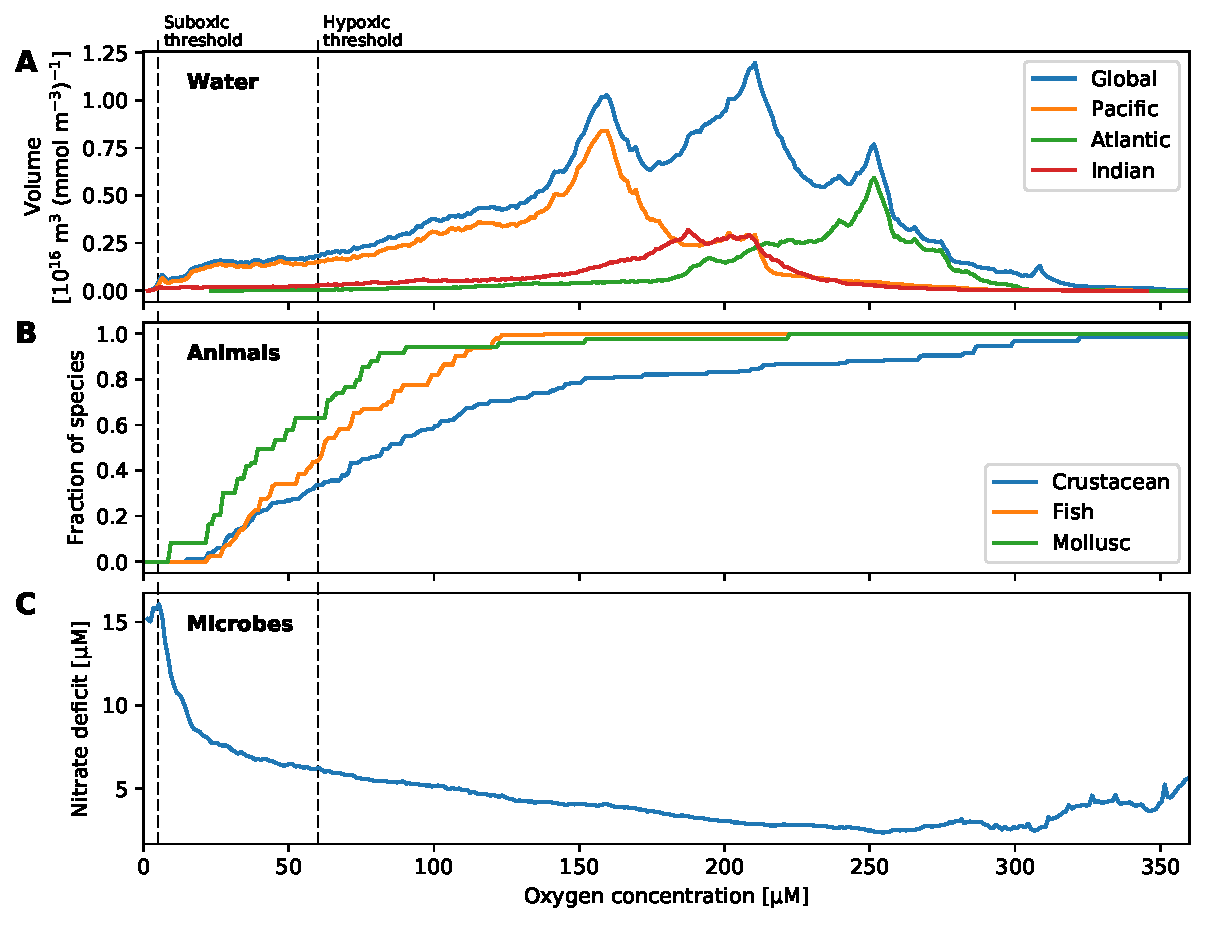
\includegraphics[width=\textwidth]{woa_o2pdf_mortality_no3deficit.pdf}
% generated by: plot_woa_o2pdf_mortality_no3deficit.ipynb
\caption{Distributions as a function of oxygen concentration:
(A) the volume of water in the global ocean, and in each major basin; (B) the fraction of species in three groups of organisms that survive at a given oxygen concentration; and (C) the nitrate deficit relative to phosphorus, defined as ${-N^* = N - r_{N:P}\ce{P}}$ \protect\citep{Gruber-Sarmiento-1997}, where ${r_{N:P}}$ is the stoichiometric ratio of remineralization of organic matter (we assume ${r_{N:P} = 16}$) \protect\citep{Anderson-Sarmiento-1994}.  Mortality thresholds are from a compilation of empirical studies \citep{Vaquer-Sunyer-Duarte-2008}.}.
\label{fig:o2pdfs}
\end{figure}
%-------------------------------------------------------------------------------

While dead zones may expand under climate warming, the impacts of ocean deoxygenation on marine macroorganisms may be more profound and widespread than suggested by projected changes in hypoxic volumes.
Indeed, the large-scale biogeographic distributions of ectothermic organisms in the contemporary ocean are limited in part by the combined effects of temperature and oxygen \citep{Deutsch-Ferrel-etal-2015}.
Metabolic rates increase in proportion to temperature; thus, an aerobic organism's demand for oxygen also increases in warmer waters.
Viable habitat is bounded by the need for a sufficient supply of oxygen to meet temperature-dependent metabolic demand.
Concomitant warming and ocean deoxygenation, therefore, can be expected to result in a contraction of metabolically viable habitat \citep{Deutsch-Ferrel-etal-2015}.
Organisms are likely to be forced poleward, where cooler waters temper oxygen demand; additionally, since oxygen concentrations typically decline with depth, we can expect a vertical habitat compression as the region of the near-surface ocean with sufficient oxygen shrinks \citep{Koslow-Goericke-etal-2011}.

%-------------------------------------------------------------------------------
\subsection{Microbes}
%-------------------------------------------------------------------------------

Just as higher animals are physiologically constrained when oxygen concentrations become low, oxygen also exerts a strong control on microbial metabolism.
When oxygen in the ocean falls below ``suboxic'' concentrations ($\ce{O2} < 5$~mmol~m$^{-3}$), aerobic metabolism becomes inefficient and microbes that use alternate electron acceptors to oxidize organic matter begin to dominate.
It may initially seem strange to worry about impinging on microbes; much of our familiarity with microbes stems from disease.
Microbes, however, play a fundamental role in sustaining all life on Earth by enabling nutrient cycling.
The importance of nutrient cycles can be appreciated by considering that the energy that powers virtually all life on Earth is harvested from the Sun during photosynthesis.
Life is carbon based---but nutrient elements such as nitrogen and phosphorus, are also fundamental building blocks required to make organic materials.
Plants and algae use sunlight to make organic matter from carbon dioxide and nutrients; they split water, use the hydrogen energy to make biomass and release \ce{O2} as waste.
The organic matter created by photosynthesis enters the food chain; primary producers are eaten by secondary producers and so on, supporting complex ecosystems.
In this manner, primary production in the ocean is the ultimate constraint on the biomass of the whole marine ecosystem.
Secondary producers have fundamentally different metabolisms than the photosynthesizers they eat; rather than producing oxygen as waste, they require oxygen to oxidize organic matter during respiration; the resulting energy is harnessed, supporting synthesis of organic matter and functional activities such as acquisition of food, growth, predator avoidance, and reproduction.
The inorganic nutrients incorporated during photosynthesis are carried up the food chain; ultimately, however, as organisms die, the organic material of which they are comprised is decomposed: microbes oxidize this material, converting its constituents back to their inorganic forms, returning nutrients to the pools upon which photosynthesis relies.
Since the ocean is a single volume of fluid, interconnected by circulation, the marine cycles of nutrients like nitrogen and phosphorus are coupled on a global scale---entering the food chain during photosynthesis, returning to dissolved inorganic forms when organic matter is ``remineralized'' via microbially-mediated oxidation.

Oxygen plays a fundamental role in these global nutrient cycles.
To illustrate this, we need to consider the fact that the cycles of nitrogen and phosphorus are regulated by fundamentally difference processes---yet organic matter is composed of nitrogen and phosphorus in specific relative amounts: more nitrogen is useless with insufficient phosphorus and vice versa.
Phosphorus is supplied to the ocean from the land via weathering and run off; it is removed from the ocean when organic material sinks and is buried in sediments.
Nitrogen, by contrast, is sourced primarily from the atmosphere, which consists of about 78\% dinitrogen gas (\ce{N2}).
Most photosynthetic organisms cannot use \ce{N2} directly, however; rather, only certain types of cyanobacteria (diazotrophs) can ``fix nitrogen,'' converting \ce{N2} gas into forms available to other organisms.
Thus, microbes determine the rate at which fixed nitrogen enters the ocean---and, as it turns out, microbes also determine the rates of removal.
As oxygen concentrations decline to suboxic levels, aerobic processes become increasingly inefficient; ultimately, when oxygen is too scarce, microbes use
other compounds as the electron acceptor needed to oxidize organic matter and make a living.
In the ocean, nitrate ($\ce{NO3}^-$) is a widespread form of fixed nitrogen; nitrate is used to oxidize organic matter in suboxic regions, converting the nitrogen to \ce{N2}, which is lost to the atmosphere.
This process is termed ``denitrification'' and it accounts for the majority of fixed nitrogen loss from the ocean \citep{Gruber-2004,Gruber-Galloway-2008}.
The signature of denitrification is evident as a ``deficit'' of nitrate relative to phosphate in suboxic regions of the global ocean (Figure~\ref{fig:o2pdfs}c).
As suboxic zones grow, the loss of fixed nitrogen to denitrification can increase, ultimately feeding back to limit primary productivity.
As ocean ecosystems are built on photosynthesis, climate-driven perturbations to oxygen that impact nutrient cycles can ultimately feedback to higher trophic levels.
Microbially-mediated processes involved in the nitrogen cycle can also have direct impacts on climate.
Denitrification and nitrification (the oxidation of ammonium to nitrate) can produce nitrous oxide (\ce{N2O}), which is an important greenhouse gas \citep{Bange-Freing-etal-2010}.
Expansion of hypoxic and suboxic volumes in the ocean may change the production and release of \ce{N2O} \citep{Nevison-Butler-etal-2003,Martinez-Rey-Bopp-etal-2015}, though this projection involves substantial uncertainty.

%-------------------------------------------------------------------------------
\subsection{Paleo-perspective}
%-------------------------------------------------------------------------------

The history of oxygen on Earth provides an important perspective on the future of oxygen in the ocean.
Indeed, for roughly the first half of Earth's 4.5 billion-year history, oxygen was not plentiful in the atmosphere; rather, significant concentrations of oxygen arose between 2.4 and 2.1 billion years ago \citep{Lyons-Reinhard-etal-2014}.
Photosynthesis is the primary source of oxygen in the atmosphere, illustrating how the evolution of life is intertwined with the character of Earth's environment: the accumulation of oxygen in the atmosphere enabled animal life, whereas prior to the evolution of photosynthesis, aerobic metabolisms were not viable.

Earth's history has been punctuated by five major extinctions, catastrophic events when more than 65\% of extant species rapidly disappeared.
The present era has been characterized as Earth's sixth mass extinction event, caused by humans and leading to irreversible changes in ecosystems \citep{Barnosky-Matzke-etal-2011}.
Some of the mechanisms driving present extinction rates are unique to the global expansion of humans---for instance, habitat fragmentation, the spread of invasive species and disease.
However, the liberation of massive amounts of geologically-sequestered carbon has happened before; thus, climate warming and the loss of ocean oxygen have well-documented analogs in the geologic record.
The end-Permian extinction, for instance, which occurred $\sim$252 million years ago, is the largest extinction event in Earth's history; nearly 95\% of terrestrial and marine species perished \citep{Raup-1979,Erwin-1993}.
Notably, the end-Permian extinction was coincident with massive volcanism, which led to elevated \ce{CO2} and climate change; extinctions in the ocean during this event can be explained by changes in oxygen levels, \ce{CO2}, and temperature \citep{Song-Wignall-etal-2014}, making this catastrophic event a compelling analog for the ocean of the 21st century \citep{Payne-Clapham-2012}.

%-------------------------------------------------------------------------------
\begin{figure}[tb]
\centering
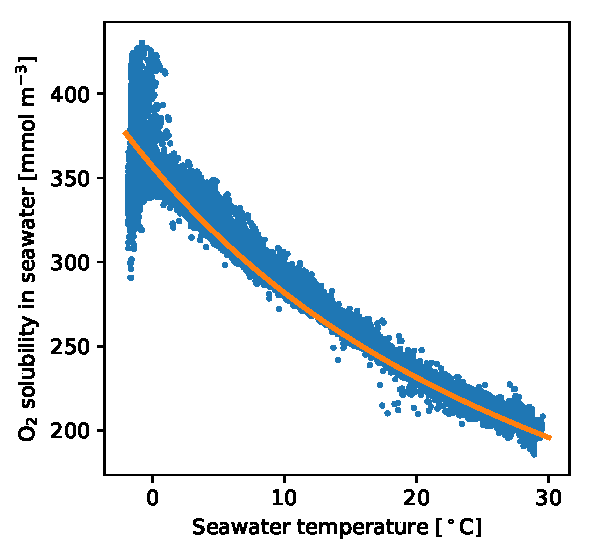
\includegraphics[width=0.4\textwidth]{o2sol-v-temp.pdf}
% generated by: plot_o2_sol.ipynb
\caption{Relationship between dissolved oxygen and temperature for surface data in the World Ocean Atlas 2013 \citep{Garcia-Locarnini-etal-2014}.
The orange line shows the saturation concentration of oxygen at equilibrium with the atmosphere \protect\citep{Garcia-Gordon-1992}.
Strong deviations from saturation are evident at near-freezing temperatures, which is partially a function of sea-ice inhibition of gas exchange \citep{Ito-Follows-etal-2004}.
}
\label{fig:o2-sol}
\end{figure}
%-------------------------------------------------------------------------------

%-------------------------------------------------------------------------------
\subsection{Climate-driven deoxygenation}
%-------------------------------------------------------------------------------

Our understanding of the basic mechanisms driving ocean deoxygenation is robust \citep{Keeling-Kortzinger-etal-2010,Gruber-2011,Bopp-Quere-etal-2002,Najjar-Keeling-2000,Plattner-Joos-etal-2002,Matear-Hirst-2003}.
Increasing concentrations of greenhouse gases, primarily carbon dioxide, trap heat in the atmosphere, leading to a planetary energy imbalance \citep{Trenberth-Fasullo-etal-2014}.
The ocean is the dominant thermal reservoir in the climate system and it is estimated that the ocean has absorbed more than 90\% of the excess heat accumulating in the Earth system since the beginning of the industrial revolution \citep{Rhein-Rintoul-etal-2013,Loeb-Lyman-etal-2012,Cheng-Trenberth-etal-2016}.
As the planet has warmed, this extra heat has accumulated in the near-surface ocean \citep{Levitus-Antonov-etal-2012,Balmaseda-Trenberth-etal-2013,Abraham-Baringer-etal-2013}.
Warmer waters hold less oxygen due to the temperature dependence of solubility; thus, as the surface ocean warms, oxygen concentrations can be expected to decline according to the solubility relationship with temperature (Figure~\ref{fig:o2-sol}).
Reductions in solubility are compounded by an additional mechanism driving deoxygenation, which involves changes to ocean circulation in response to warming.
The density of seawater is strongly temperature dependent; warmer waters are less dense or, equivalently, more buoyant.
As extra heat is absorbed by the ocean, it tends to warm the surface ocean at a greater rate than warming at depth, increasing the density difference between surface and deep water.
This enhanced density stratification inhibits exchange between the oxygen-rich surface ocean and waters in the interior where oxygen is consumed by respiration.
Diminished surface-to-depth exchange reduces the quantity of oxygen supplied to the ocean interior, shifting the balance maintaining oxygen concentrations: consumption exceeds supply, oxygen concentrations decline.
This reinforcing mechanism, wherein temperature-related solubility effects are amplified by the effect of density stratification, makes oxygen exceptionally sensitive to variations in climate.
However, the enhanced stratification and slower circulation of the upper ocean has a countervailing effect: it simultaneously reduces the supply of nutrients from deep waters to the photic zone, reducing productivity at the surface and ultimately the respiration of organic matter below.
The reduced oxygen demand offsets part of the reduced supply.
This compensating mechanism, in concert with the reinforcing mechanism noted above, creates the potential for complex regional and time-scale dependent behavior in the \ce{O2} changes.
Indeed, as we shall see below, dissolved oxygen is highly dynamic in the present-day climate, exhibiting dramatic variations on annual to multi-decadal timescales \citep{Ito-Deutsch-2010,Deutsch-Brix-etal-2011}.
These natural fluctuations in oxygen drive important shifts in marine ecology and biogeochemistry \citep[e.g.,][]{Rabalais-Diaz-etal-2010,Zamora-Oschlies-etal-2012,Deutsch-Berelson-etal-2014,Yang-Gruber-etal-2016}---and yet over the next century, the amplitude of oxygen changes is likely to be much greater, far exceeding the range of natural variability \citep{Long-Deutsch-etal-2016,Rodgers-Lin-etal-2015,Henson-Beaulieu-etal-2017}.

%-------------------------------------------------------------------------------
\subsection{Earth system models}
%-------------------------------------------------------------------------------

While the basic mechanisms controlling deoxygenation are well-understood in principle, details of ocean circulation and biological productivity lead to regional differences in the rate and magnitude of oxygen loss.
In this chapter, we discuss projections of ocean oxygen under future emissions scenarios.
Our most sophisticated tools in this enterprise are Earth system models (ESMs); these consist of coupled atmosphere and ocean general circulation models (GCMs) and include representations of processes relevant to ocean biogeochemistry.
Our objectives are to review the state of knowledge regarding the rate, magnitude and geographic distribution of expected deoxygenation trends, relying primarily on ESM projections.

To illustrate both the robust and uncertain projections for future ocean oxygen, we will present results from two primary collections of model solutions.
First, we make use of a large ensemble of a single, fully-coupled ESM: the Community Earth System Model (CESM).
The CESM Large Ensemble (CESM-LE) has more than 30 independent realizations of the historical period from 1920--2005 and future projections out to 2100 under  the CMIP5 ``business-as-usual'' RCP8.5 forcing scenario \citep{Kay-Deser-etal-2015}.
Second, we show results from a subset of the CMIP5 multi-model ensemble, enabling perspective on the degree to which CESM is representative of this broader collection of independently developed models.
The models are from the Geophysical Fluid Dynamics Laboratory (GFDL) \citep{Dunne-John-etal-2012a,Dunne-John-etal-2013b}; the UK Met Office Hadley Centre (HadGEM) \citep{Collins-Bellouin-etal-2011,HadGEM2-Development-Team-2011}; the Max Planck Institute (MPI) \citep{Giorgetta-Jungclaus-etal-2013}; and the Institut Pierre Simon Laplace (IPSL) \citep{Dufresne-Foujols-etal-2013}.
We also include CESM's CMIP5 solutions \citep{Hurrell-Holland-etal-2013}; this model is similar to the CESM-LE in many respects, but has a different atmospheric model so does display distinct behavior.

The ``spread'' across the CESM-LE and the CMIP5 ensembles reflects different sources of uncertainty \citep{Hawkins-Sutton-2009}.
Internal variability is an intrinsic feature of the climate system, arising from nonlinear dynamical processes and interactions between the ocean, atmosphere and land surface that each integrate forcing over different timescales \citep{Hasselmann-1976}.
Earth system models generate internal climate variability representative of that in nature, thus the ensemble spread of the CESM-LE can be used to assess the contribution of natural variability to uncertainty in future projections, which is particularly important on regional scales \citep{Deser-Phillips-etal-2012,Lovenduski-McKinley-etal-2016,McKinley-Pilcher-etal-2016}.
While internal climate variability contributes to the spread in the CMIP5 ensemble, each of the models in this collection has distinct behavior reflecting differences in underlying formulations.
Thus, spread across the CMIP5 models reflects a minimum bound on the contribution of ``structural uncertainty'' to future projections \citep{Hawkins-Sutton-2009,Lovenduski-McKinley-etal-2016}.
Finally, human activity introduces substantial uncertainty into future projections.
Indeed, the magnitude of surface warming during the next century is strongly dependent on the amount of greenhouse gases emitted over the next several decades \citep{Collins-Knutti-etal-2013}.
To account for this source of uncertainty, CMIP5 included four ``Representative Concentration Pathway'' scenarios intended to span a range of total radiative forcing at 2100 from 2.6~W~m$^{-2}$ (RCP2.6) to 8.5~W~m$^{-2}$ (RCP8.5) \citep{Meinshausen-Smith-etal-2011}.
The differences in these scenarios illustrate the contribution of ``scenario uncertainty'' to future projections.
Our primary focus will by on the RCP8.5 scenario, but we include limited results from RCP4.5 and discuss the benefits of climate change mitigation activities to the ocean deoxygenation problem \citep{Henson-Beaulieu-etal-2017}.

%-------------------------------------------------------------------------------
\section{Understanding dissolved oxygen}\label{loc:o2-distributions}
%-------------------------------------------------------------------------------

%-------------------------------------------------------------------------------
\begin{figure}[p!]
\centering
\includegraphics[width=1\textwidth]{schematic-w2.pdf}
% generated by: illustrator
\caption{Schematic illustration of the mechanisms controlling oxygen distributions in the ocean.
Oxygen is produced in the surface ocean by biological productivity, which generates organic matter.
Air-sea exchange keeps oxygen in the surface ocean near saturation concentrations with the atmosphere ($\ce{O2}^{sat}$).
Oxygen is consumed in the interior as organic matter is respired; the rate of oxygen consumption is termed the ``oxygen utilization rate'' ($OUR$).
``Apparent oxygen utilization'' (${AOU = \ce{O2}^{sat} - \ce{O2}}$) provides an estimate of the amount of oxygen that has been consumed by respiration as a water parcel circulates in the ocean interior.
Illustration by Matthew Long and Ryan Johnson (NCAR).}
\label{fig:schematic}
\end{figure}
%------------------------------------------------------------------------------

Several concepts are required to understand the mechanisms driving ocean deoxygenation.
To review these, we first examine the large-scale structure of present-day oxygen distributions.
An understanding of the basic physical and biological controls on these distributions provides perspective on the mechanisms by which climate warming drives oxygen loss.
Our primary resource for understanding the global scale ocean oxygen distributions come from the World Ocean Atlas (WOA), produced by the National Oceanographic Data Center (United States).
WOA is a compilation of observations that have been objectively-analyzed to produce gridded fields at a spatial resolution of 1$^\circ\times1^\circ$.
While we only consider annual-mean distributions here, WOA includes monthly data, enabling evaluation of the seasonal cycle.
The observations upon which WOA is based, however, do not have sufficient coverage to enable a globally gridded-product with temporal resolution beyond the monthly mean annual cycle.
Thus, efforts to evaluate global-scale trends in \ce{O2} based on observations (section~\ref{loc:obs-tr}) have relied on independently-developed compilations of observations \citep[e.g.,][]{Helm-Bindoff-etal-2011,Ito-Minobe-etal-2017,Schmidtko-Stramma-etal-2017}.

As discussed in section~\ref{loc:intro}, oxygen is supplied to the ocean via exchange with the atmosphere and photosynthetic oxygen production at the surface.
The ocean surface, therefore, tends to be well-oxygenated---which is to say the concentration of oxygen remains near the saturation concentration ($\ce{O2}^{sat}$) with respect to the atmosphere.
Photosynthesis in the surface ocean produces organic matter; detrital remnants of this material sink to depth where they are broken down by microbial respiration, consuming oxygen (Figure~\ref{fig:schematic}).
Thus, oxygen concentrations are elevated where freshly subducted surface waters flow into the interior, but concentrations decline downstream of these regions as a respiration signal accumulates.
Large-scale patterns are set by the global overturning circulation, wherein oxygen is supplied to the ocean in ventilation regions, and is subsequently depleted as waters circulate in the interior.
In the upper ocean thermocline, where respiration rates are relatively fast, oxygen concentrations span a range from full saturation at the surface to near zero at the tropical terminus (Figure~\ref{fig:woa-thermocline-o2-age}).
In the abyssal ocean, where respiration rates are very slow, the high \ce{O2} values obtained in polar surface waters decline to intermediate values at the end of the great ocean conveyor in the Pacific \citep{Broecker-1991}.

%-------------------------------------------------------------------------------
\begin{figure}[t!]
\centering
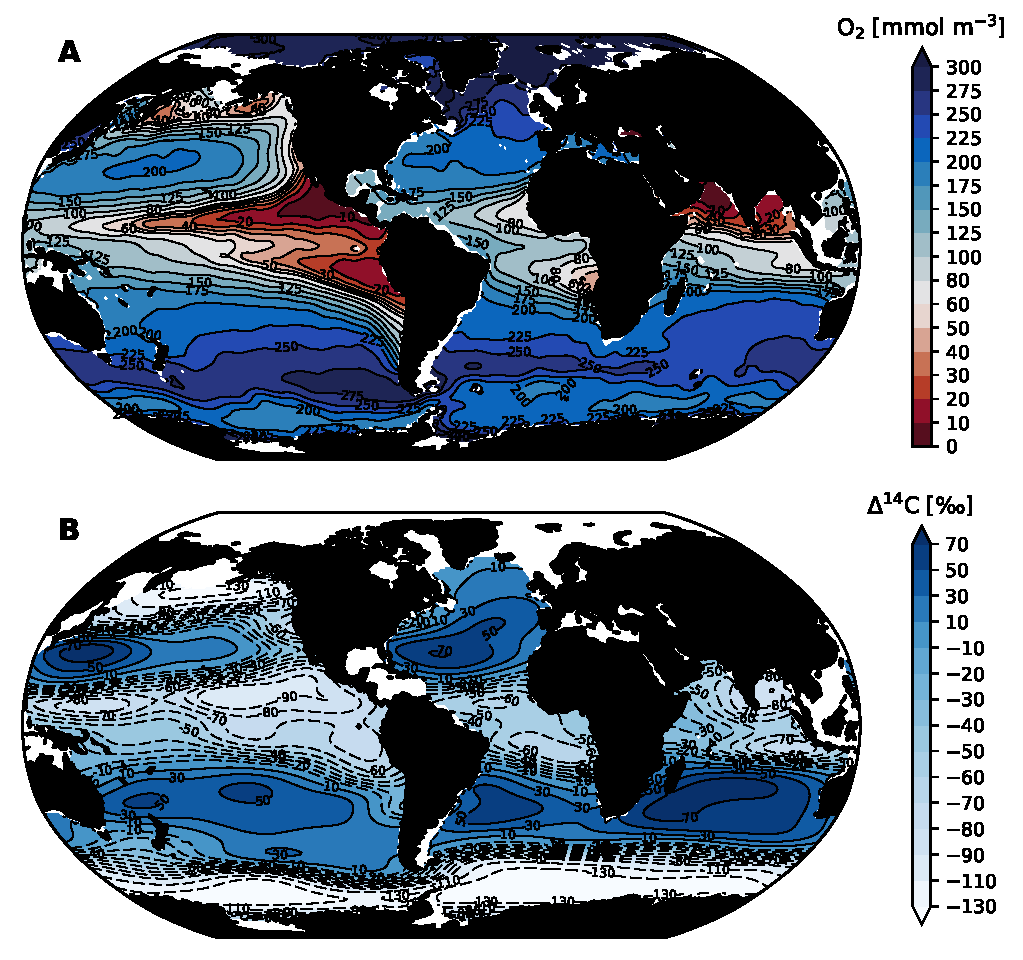
\includegraphics[width=0.8\textwidth]{woa-thermocline-o2-w-age_metric.pdf}
% generated by: plot_woa_thermocline_o2_and_age_metric.ipynb
\caption{Oxygen distributions and a metric of water mass age averaged over 200--600~m depth based on observations.
(A) The average dissolved oxygen concentration from the World Ocean Atlas, 2013, version 2 \citep{Garcia-Locarnini-etal-2014}; regions plotted in red are below 60~mmol~m$^{-3}$, which is a common definition for an hypoxic threshold.
(B) Total radiocarbon concentrations ($\Delta$\ce{^{14}C}) from the Global Data Analysis Project (GLODAP) data synthesis \protect\citep{Key-Kozyr-etal-2004}.
Low $\Delta$\ce{^{14}C} is indicative of older waters; since these waters have been isolated from the atmosphere for longer, they are depleted in natural \ce{^{14}C} and contain limited anthropogenic \ce{^{14}C}.
Most of the spatial structure in the total radiocarbon field at these depths is from the anthropogenic or ``bomb'' component \citep{Key-Kozyr-etal-2004}.}
\label{fig:woa-thermocline-o2-age}
\end{figure}
%-------------------------------------------------------------------------------

The ``age'' of waters in the ocean interior is a useful metric to consider in the context of ocean ventilation; age can be defined as the time since waters last contacted the surface.
As waters grow older in the ocean interior, oxygen is continually depleted by respiration; the accumulated impact of this consumption is termed Apparent Oxygen Utilization and is estimated based on the difference from saturation ($AOU = \ce{O2}^{sat} - \ce{O2}$), assuming that the oxygen concentration was close to $\ce{O2}^{sat}$ at the time of subduction \citep{Ito-Follows-etal-2004}.
Thus, $AOU$ is an estimate of the amount of respiration integrated along the path waters take as they circulate in the ocean interior.
Older waters can be expected to have greater $AOU$, and hence lower oxygen, because they have spent a longer time accumulating a respiration signal.
This explains the contrast between dissolved oxygen concentrations in the thermocline of the North Pacific versus North Atlantic, for instance (Figure~\ref{fig:woa-thermocline-o2-age}).
Freshly formed deep water fills the North Atlantic basin; this water is rich in oxygen from recent surface exchange and, as there is only modest accumulation of a respiration signal, it remains relatively close to saturation concentrations (low $AOU$).
The North Pacific, by contrast, is the last stop on the great ocean conveyor and as a result, deep water in this basin is substantially depleted in oxygen (Figure~\ref{fig:woa-o2-column-min}).
Mode water ventilation in the western North Pacific supplies oxygen to the subtropical thermocline, but the thermocline on the eastern side of the basin is characterized by strong oxygen depletion (Figure~\ref{fig:woa-thermocline-o2-age}).
An examination of the global distributions of radiocarbon ($\Delta\ce{^{14}C}$) in the thermocline depth range confirms that water mass age is a dominate control on oxygen: old waters are highly depleted in \ce{^{14}C} since they have been isolated from the atmosphere for longer; these waters have had longer to accumulate $AOU$, and thus tend to be more depleted in oxygen (Figure~\ref{fig:woa-thermocline-o2-age}).

%-------------------------------------------------------------------------------
\begin{figure}[tbp]
\centering
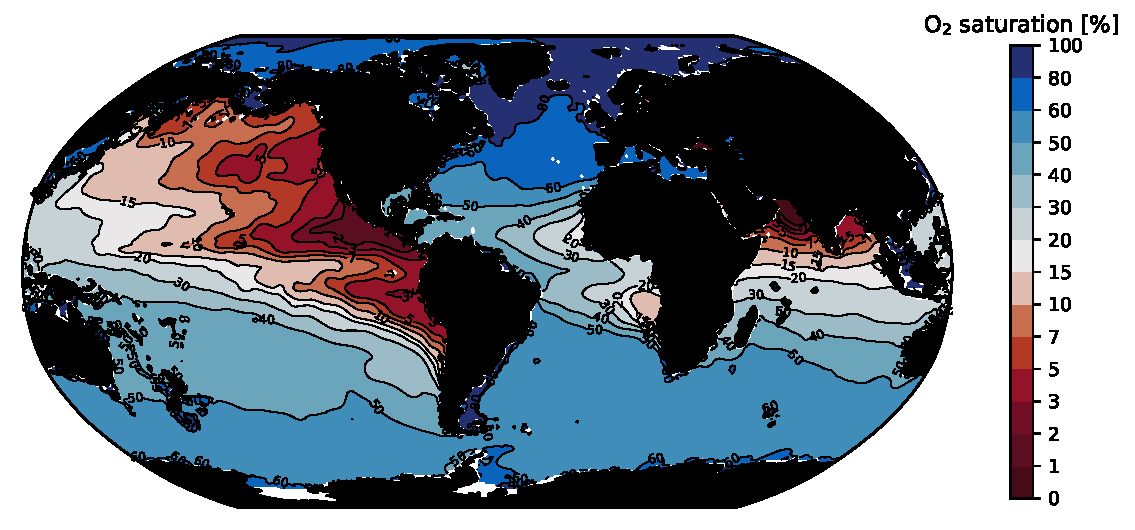
\includegraphics[width=0.8\textwidth]{woa-column-min-o2-sat.pdf}
% generated by: plot_woa_maps.ipynb
\caption{Oxygen saturation at the point in the vertical column where oxygen saturation is minimum; computed from the World Ocean Atlas, 2013, version 2 \protect\citep{Garcia-Locarnini-etal-2014}.
Saturation values less than 15\% are colored in red.}
\label{fig:woa-o2-column-min}
\end{figure}
%-------------------------------------------------------------------------------

The age of water dictates the time available to accumulate a respiration signal in the form of oxygen depletion; however, the rate at which oxygen is depleted by respiration---or, equivalently, the rate at which $AOU$ increases---can also vary.
In particular, $AOU$ increases at a rate that is largely proportional to the quantity of organic matter being respired.
Regions with greater inputs of organic matter will have higher oxygen utilization rates ($OUR$), which drive faster increases in $AOU$.
Depth is a dominant control on $OUR$ because the downward flux of organic matter decreases approximately exponentially with depth.
Most sinking organic matter is respired in the upper 1,000~m of the ocean, leading to higher $OUR$ there; oxygen demand in deep waters is relatively low.
This remineralization profile is an important driver of ``oxygen minimum zones'' (OMZs), which are regions of very low oxygen found on the eastern side of the ocean basins in the tropics (highlighted in red on Figure~\ref{fig:woa-thermocline-o2-age}a).
Oxygen concentrations approach zero in the core of the OMZs because the rate of fresh oxygen supply via mixing and advection cannot match the rate of organic matter consumption.
As discussed above, oxygen minimum zones play an important role in global biogeochemical cycles of nutrients; in particular, nitrogen.
As oxygen declines, a larger fraction of the oxidation of nitrogen in organic matter is shunted to \ce{N2O}, increasing the concentrations of this greenhouse gas in hypoxic waters.
As \ce{O2} is depleted to near zero concentrations, nitrate becomes the dominant electron acceptor used to oxidize organic matter, resulting in a loss of fixed nitrogen from the ocean; microbial communities also switch from \ce{N2O} production to consumption when \ce{O2} is very low \citep{Codispoti-2010}.

As we have already said, climate warming drives deoxygenation via two pathways.
The first is straightforward and involves reductions in thermal solubility of gases.
The second is less straightforward; it includes the role of diminished ventilation (Figure~\ref{fig:schematic}) that results from density stratification.
As ventilation declines, the age of waters in the ocean interior increase, leading to an increase in $AOU$.
Notably, the same processes involved with ventilation play a role in sustaining surface ocean primary productivity.
Primary productivity operates in the sunlit-surface layer of the ocean (the euphotic zone); nutrients are consumed in the process of carbon fixation, and ultimately exported to depth where they are remineralized; this collection of processes is referred to as the ``biological pump'': it ``pumps'' carbon into the deep ocean in spite of the homogenizing influence of circulation \citep{Volk-Hoffert-1985}.
The biological pump is dependent on vertical mixing and advection to return nutrients from depth back into the surface layer; warming-driven stratification will curtail this nutrient supply, just as it does for the delivery of fresh oxygen to the interior ocean.
Stratification, therefore, is expected to lead to a reduction in surface ocean primary production \citep{Steinacher-Joos-etal-2010,Bopp-Resplandy-etal-2013}, which will very likely have significant consequences for marine ecosystems and the fisheries they support \citep{Stock-John-etal-2017}.
A reduction in the biological pump alleviates some demand for oxygen in the interior via reducing $OUR$; this effect, however, is not expected to fully compensate for the reduced ventilation because in regions with unused surface nutrients, a slower circulation need not slow the rate of organic matter production.
Since stratification increases the residence time of surface waters, primary productivity is able to effect a more complete utilization of nutrients in the surface layer.
It is useful to consider the partitioning of nutrients, such as phosphate, into preformed and regenerated pool.
The ``preformed'' phosphate, for instance, refers to the phosphate concentration at the time of water mass formation---when the water first subducts in the ocean interior.
In contrast, ``regenerated'' phosphate is closely related to $AOU$ as it accounts for the cumulative (or path-integrated) amount of phosphate released by the microbial decomposition of organic matter since the water mass entered the interior.
As nutrient utilization in the surface ocean becomes more complete, ``preformed'' concentrations of nutrients in waters sinking into the ocean interior decline.
Practically, the oceanic inventory of phosphate can be treated as constant on timescale of tens of thousands of years, so the global sum of preformed and regenerated phosphate must be conserved; therefore, the decline in preformed phosphate must be compensated by an increase in remineralized (or regenerated) phosphate.
On this basis, stratification can be expected to yield an increase in $AOU$ and an associated decrease in oxygen.

%-------------------------------------------------------------------------------
\subsection{Observed trends}\label{loc:obs-tr}
%-------------------------------------------------------------------------------

A few studies have examined oxygen distributions on a global scale and found declines that appear consistent with expectations based on model simulations.
\citet{Helm-Bindoff-etal-2011} found a globally-averaged decrease in upper-ocean (100--1000~m) oxygen an inventory trend of $-55 \pm 13$~Tmol~yr$^{-1}$ (1~Tmol = $10^{12}$~mol).
This is consistent with \citet{Manning-Keeling-2006}, who found a net oxygen outgassing from the ocean over the period  1993--2003 of $-45$~Tmol~yr$^{-1}$.
\citet{Schmidtko-Stramma-etal-2017} reported somewhat larger numbers analyzing data from full depth over the period 1960--2015, finding trends in the oxygen inventory of $-96.1\pm42.9$~Tmol~yr$^{-1}$.
\citet{Ito-Minobe-etal-2017}, using a different compilation of similar datasets, found a trend of $-24.3\pm12.4$~Tmol~yr$^{-1}$ over the upper 1000~m.
Data coverage is a major limitation in assessing global trends; however, the observed changes are not inconsistent with the changes expected from anthropogenic warming.
Notably, observationally-based studies have found that direct solubility effect can account for about 15\% of oxygen declines \citep{Helm-Bindoff-etal-2011,Schmidtko-Stramma-etal-2017}, which is significantly less than modeling studies have found \citep[e.g.,][]{Bopp-Quere-etal-2002}.

While global data coverage is difficult to achieve, one might imagine that sufficiently long time series exist in particular oceanic regions, thereby enabling detection and attribution of forced trends.
Indeed, many studies have evaluated low-frequency variability and long-term trends in local to regional scale \ce{O2} observations, including at ocean time series sites \citep[e.g.,][]{Ono-Midorikawa-etal-2001,Andreev-Baturina-2006,Whitney-Freeland-etal-2007,McClatchie-Goericke-etal-2010}, repeat hydrographic sections \citep[e.g.,][]{Emerson-Watanabe-etal-2004,Johnson-Gruber-2007,Mecking-Langdon-etal-2008,van-Aken-Femke-de-Jong-etal-2011,Sasano-Takatani-etal-2015} or compilation and optimal interpolation of historic observations \citep[e.g.,][]{Stramma-Johnson-etal-2008,Helm-Bindoff-etal-2011,Stendardo-Gruber-2012}.
While statistically significant trends in interior oxygen distributions have been observed in specific oceanic regions, and in some cases over long time periods (50 years) \citep{Stendardo-Gruber-2012}, definitive attribution of these trends to externally-forced climate change is challenged by the presence of significant background `noise' associated with internally-driven, low-frequency climate variability \citep{Garcia-Boyer-etal-2005,Ito-Deutsch-2010}.

%-------------------------------------------------------------------------------
\section{Future projections}
%-------------------------------------------------------------------------------

Just as the distribution of oxygen in the modern ocean can be understood on the basis of the combined influences of temperature, ventilation rates, and patterns of oxygen consumption, the future of dissolved oxygen can be predicted on the basis of expected perturbations in these factors.
The proximal driver of these perturbations is the warming of the ocean, thus we fist examine expected changes in ocean heat content and its impact on stratification.

%-------------------------------------------------------------------------------
\begin{figure}[tb]
\centering
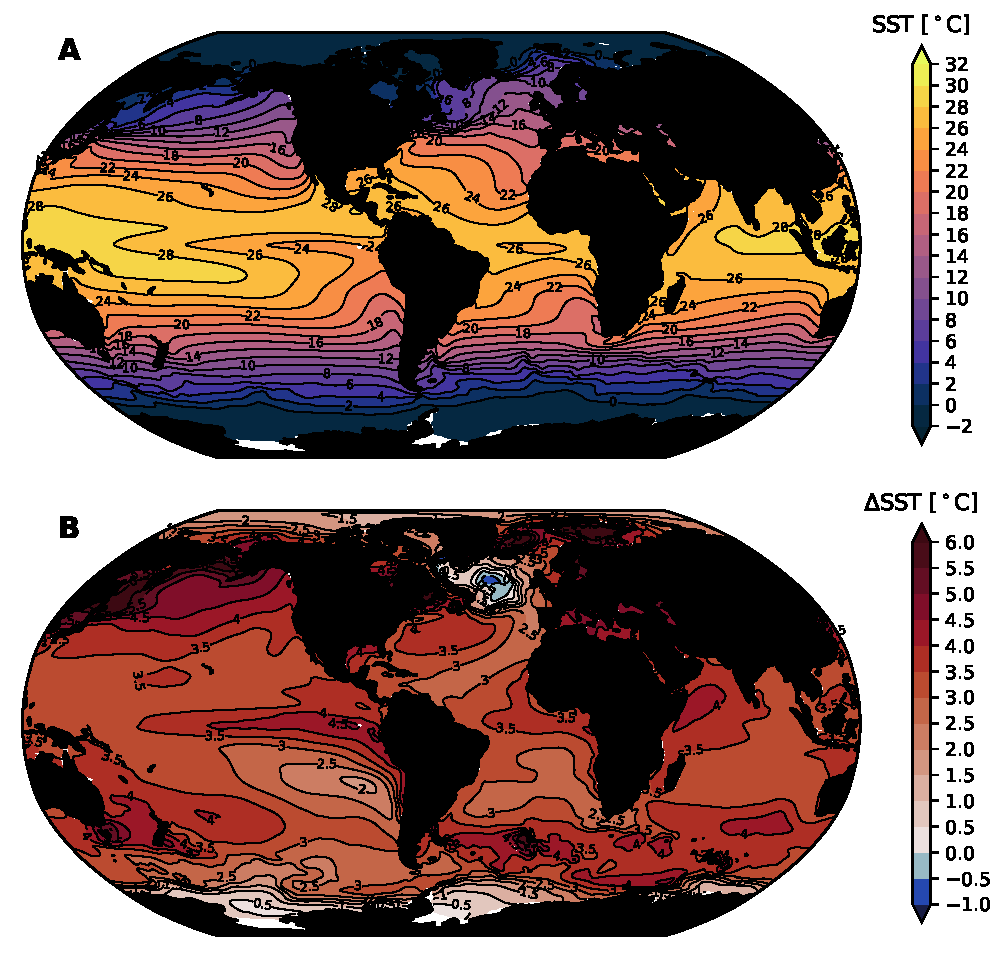
\includegraphics[width=0.75\textwidth]{cesm-sst.pdf}
% generated by: plot_global_timeseries.ipynb
\caption{(A) Ensemble-mean sea surface temperature (SST) in the mean climate and (B) the change in SST at the year 2100 as simulated by the CESM-LE \protect\citep{Kay-Deser-etal-2015}.}
\label{fig:cesm-temp-change}
\end{figure}
%-------------------------------------------------------------------------------

%-------------------------------------------------------------------------------
\subsection{Ocean heat uptake}\label{loc:heat-uptake}
%-------------------------------------------------------------------------------

%-------------------------------------------------------------------------------
\begin{figure}[tbp]
\centering
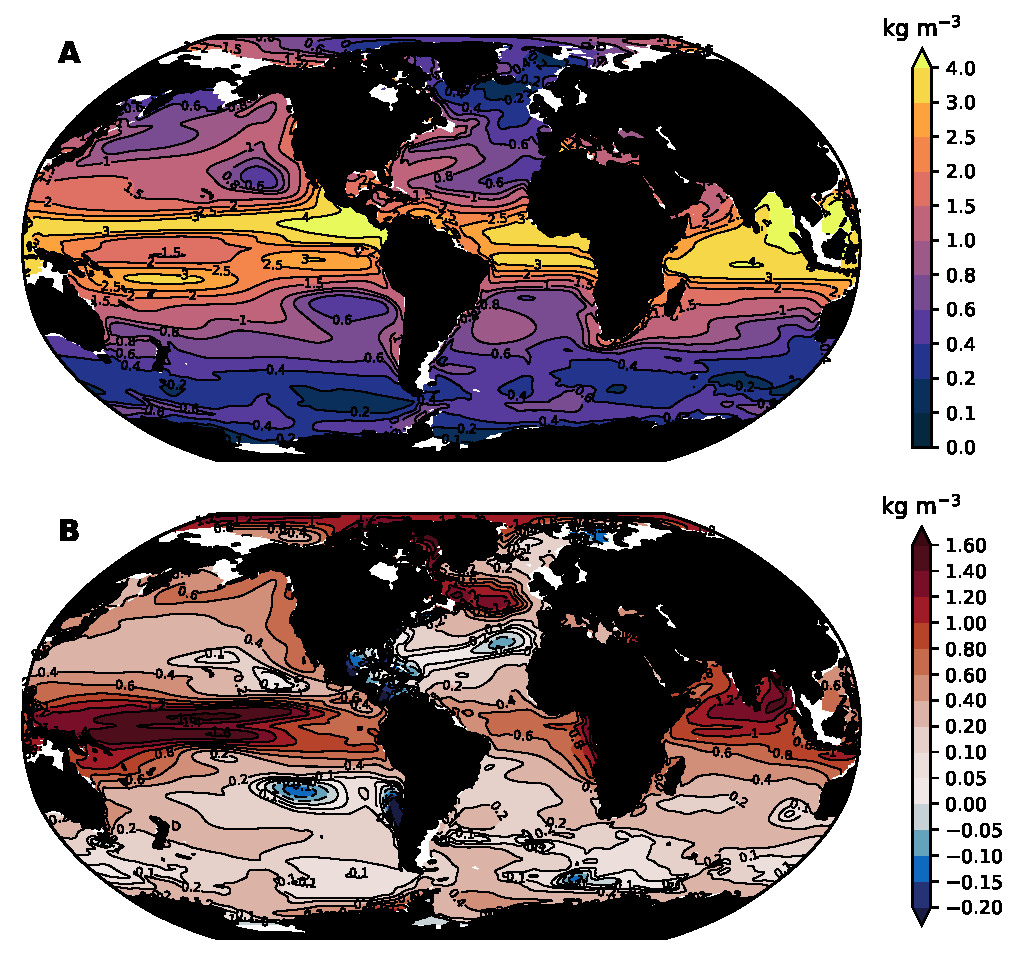
\includegraphics[width=0.8\textwidth]{cesm-stratification.pdf}
% generated by: plot_cesm_zonal_sections.ipynb
\caption{Upper ocean stratification: (A) Density difference between the upper-ocean (0--50~m) and upper-thermocline (100--200~m) in the mean climate from the CESM-LE; (B) changes in stratification at 2100.}
\label{fig:cesm-stratification}
\end{figure}
%-------------------------------------------------------------------------------

In each of the CMIP5 scenarios (RCP2.6, RCP4.5, RCP6.0 and RCP8.5), increasing atmospheric carbon dioxide (\ce{CO2}) concentrations is the dominant driver of changes in radiative forcing, accounting for about 80--90\% of the total anthropogenic influence on climate \citep{Collins-Knutti-etal-2013}.
%, with the largest changes in upper-ocean temperature projected in tropical and subtropical regions.
All scenarios result in substantial warming of the ocean, which moderates the effect of climate change on land, but results in impacts on sea level rise and ocean circulation \citep{Gattuso-Magnan-etal-2015}.
The CMIP5 collection of models suggests that at 2100, the top 100~m of the ocean will have warmed by about 0.6$^\circ$C under RCP2.6 and up to 2.0$^\circ$C under RCP8.5 relative to preindustrial \citep{Collins-Knutti-etal-2013}.
Figure~\ref{fig:cesm-temp-change} illustrates the distribution of sea surface temperature (SST) change in the CESM-LE under RCP8.5; there is a near-ubiquitous increase in tropical and subtropical SSTs by 3--4$^\circ$C and very strong warming in the Subarctic North Pacific.
A ``warming hole'' appears in the North Atlantic, a feature associated with reduced meridional overturning circulation that limits northward heat transport \citep{Drijfhout-Oldenborgh-etal-2012}.

The distribution of warming in future projections is consistent with an amplification of observed patterns of temperature change \citep{Levitus-Antonov-etal-2012} and manifests in part from ocean circulation.
Low latitude oceans are relatively well-stratified (Figure~\ref{fig:cesm-stratification}a), which inhibits mixing and advection of heat away from the surface and into the ocean interior; heat trapped in surface waters drives large temperature increases.
High-latitude regions tend to be weakly stratified, by contrast, leading to smaller changes in temperature as heat is mixed over a larger volume of ocean.
The Southern Ocean is exceptional in this regard; recent decades have been marked by little surface warming in this region, explained by upwelling and subsequent northward advection of deep water \citep{Armour-Marshall-etal-2016}.

A key feature of the ocean warming expected under future scenarios is that it is strongly surface intensified.
Half of the excess heat absorbed by the ocean at 2100 under RCP4.5, for instance, is expected to be confined to the upper 700~m of the water column \citep{Collins-Knutti-etal-2013}.
This is expected on the basis of theoretical understanding of ocean response timescales to transient forcing \citep{Held-Winton-etal-2010,Stouffer-2004}.
The mixed layer in the surface ocean responds rapidly to changes in radiative forcing in the atmosphere, but the deep ocean requires millennia to equilibrate \citep{Hansen-Sato-etal-2011,Li-Storch-etal-2013}.
A consequence of this vertical progression of warming is a strong increase in upper ocean stratification, particularly while transient forcing remains in effect \citep{Xu-Xie-etal-2012,Xu-Xie-etal-2013}.
Figure~\ref{fig:cesm-stratification}b shows the change in upper ocean stratification simulated by the CESM-LE.
The change in stratification is strongest in the tropics and in the Arctic Ocean; there are widespread increases in stratification at mid- to high-latitudes, with some localized and weak reductions in stratification.
Stratification in the Subarctic North Pacific is expected to increase dramatically.
The ``warming hole'' in the North Atlantic is associated with a strong increase in stratification, confirming that this feature involves substantial changes in freshwater content that accompanies cooling.

%-------------------------------------------------------------------------------
\subsection{Global oxygen declines}
%-------------------------------------------------------------------------------

%-------------------------------------------------------------------------------
\begin{figure}[tbp]
\centering
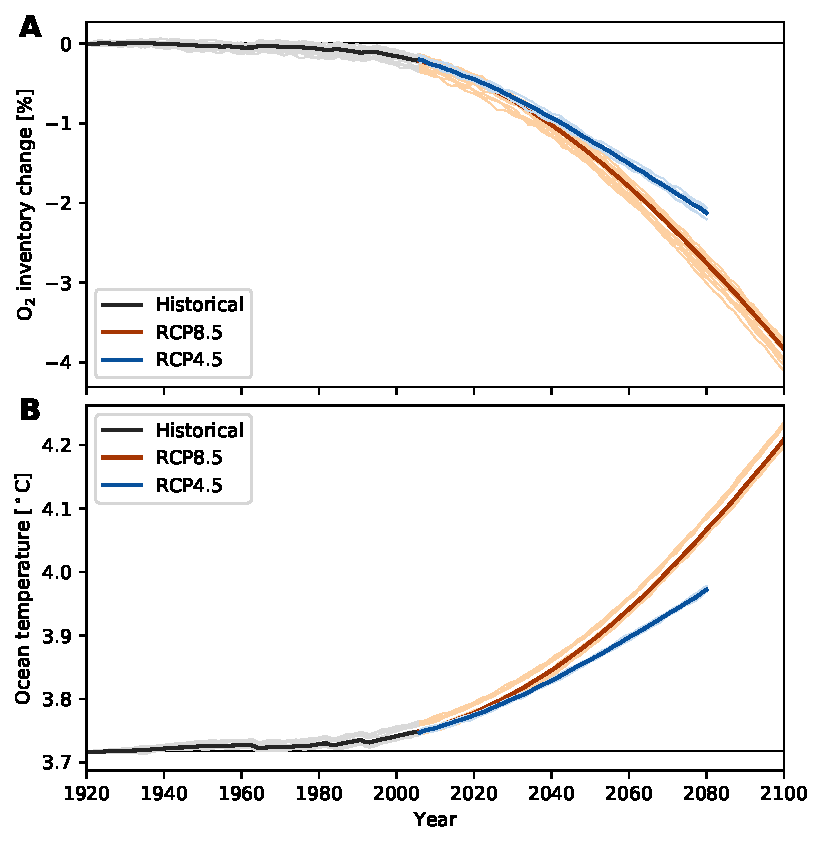
\includegraphics[width=0.75\textwidth]{cesm-global-timeseries.pdf}
% generated by: plot_global_timeseries.ipynb
\caption{Change in global-mean ocean properties as simulated in the Community Earth System Model Large Ensemble (CESM-LE): (A) percent change the ocean oxygen inventory relative to the ``control'' climate; and (B) ocean temperature.
Red lines show results from RCP8.5, blue lines show results from RCP4.5 (blue).
We use the ensemble mean over the period 1920--1939 to define the ``control'' climate.}
\label{fig:cesm-global-timeseries}
\end{figure}
%-------------------------------------------------------------------------------

Earth system model simulations indicate that the global ocean will begin to lose oxygen at an accelerating rate in the early 21st century, with a tight correspondence to increases in ocean heat content \citep{Bopp-Resplandy-etal-2013}.
This phenomenon is illustrated in Figure~\ref{fig:cesm-global-timeseries}, which shows results from the CESM-LE, including RCP8.5 and RCP4.5 scenarios.
In these simulations, oxygen declines are evident in the late 20th century, but rates of change strongly increase in the early to mid 21st century.
Notably, ensemble spread is limited at the global scale; this is because spatial averaging reduces the contribution of natural variability to trends, leaving a signal that is mostly driven by external forcing.
Differences between RCP8.5 and RCP4.5 start to become evident for global ocean temperature around 2040, but manifest somewhat later for global \ce{O2}, reflecting, in part, the greater variability (ensemble spread) in the simulated \ce{O2} inventory relative to temperature.

The acceleration in the rate of oxygen depletion is a common feature across the CMIP5 models \citep{Bopp-Resplandy-etal-2013,Cocco-Joos-etal-2013}.
In the CESM-LE under RCP8.5 (Figure~\ref{fig:cesm-global-timeseries}a), the ensemble mean trend in the global-ocean oxygen inventory during the first two decades of the 21st century increased in magnitude from about $-$20~Tmol~yr$^{-1}$ to nearly $-$60~Tmol~yr$^{-1}$.
By mid-century (2050s), the model suggests that the ocean will be losing about 100~Tmol of oxygen per year and this rate of loss will continue to increase to more than 130~Tmol~yr$^{-1}$ by the end of the century.
Notably, however, \citet{Schmidtko-Stramma-etal-2017} reported an observationally-based estimate of the rate of oxygen loss between 1960--2015 that was about $-$100~Tmol~yr$^{-1}$.
This suggests that models may underestimate the true deoxygenation rates.
The reasons for this discrepancy are not fully understood, but there are indications that stong trends observed in the tropical oceans \citep{Stramma-Johnson-etal-2008,Stramma-Oschlies-etal-2012} are not replicated in many simulations \citep{Oschlies-Duteil-etal-2017}.


%-------------------------------------------------------------------------------
\begin{figure}[tbp]
\centering
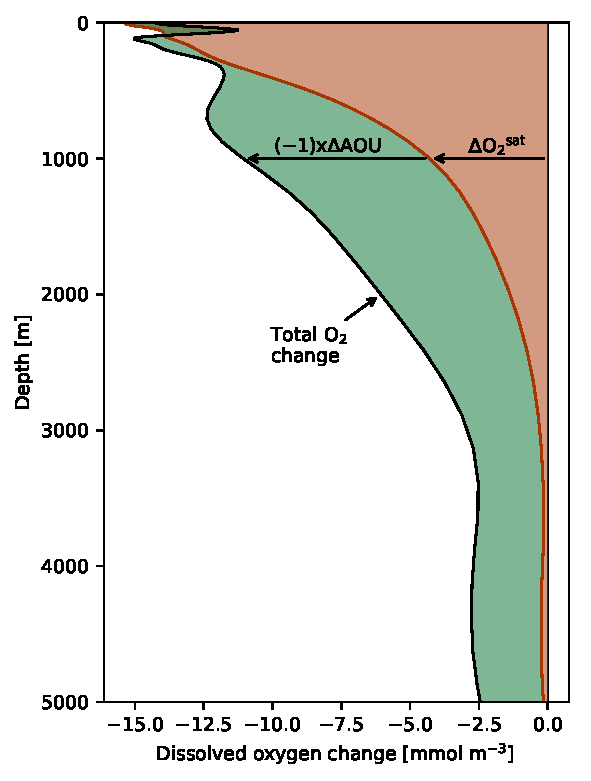
\includegraphics[width=0.6\textwidth]{cesm-o2-change-profile.pdf}
% generated by: plot_cesm_zonal_sections.ipynb
\caption{Mechanisms driving global oxygen change in the CESM-LE.
The total oxygen decline (black) and the contribution of reduced solubility (orange area) and increase respiration ($\Delta$AOU, green area).
We use the ensemble mean over the period 1920--1939 to define the ``control'' climate.}
\label{fig:cesm-global-profile}
\end{figure}
%-------------------------------------------------------------------------------

The global-scale \ce{O2} declines depicted in Figure~\ref{fig:cesm-global-timeseries} result from a combination of the direct warming-induced reduction in solubility and changes cumulative respiration brought about by stratification.
Changes in respiration can be quantified by changes in $AOU$, presuming that oxygen in the surface ocean remains relatively close to saturation.
As explained above, an increase in $AOU$ indicates greater path-integrated respiration, which corresponds to a decrease in the oxygen concentration.
Therefore, the total change in oxygen concentrations under climate warming, $\Delta\ce{O2}$, can be written as the sum of changes due to warming effects on saturation concentrations ($\Delta\ce{O2}^{sat}$) and respiration effects quantified by the negative of changes in $AOU$ ($-\Delta AOU$):
\begin{equation}
\Delta\ce{O2} = \Delta\ce{O2}^{sat} - \Delta AOU.
\label{eqn:o2-change}
\end{equation}

Figure~\ref{fig:cesm-global-profile} illustrates this interplay of mechanisms driving oxygen loss for a global-mean vertical profile computed from the CESM-LE.
The total global \ce{O2} change at 2100 ($\Delta\ce{O2}$) is shown as a black line; the contribution of changes in oxygen solubility ($\Delta\ce{O2}^{sat}$) and respiration ($-\Delta{}AOU$) are highlighted with orange and green shading, respectively.
Oxygen depletion is strongest in the upper 1000~m, exceeding $-$10 mmol m$^{-3}$ over this depth range.
Solubility-driven declines in oxygen decay rapidly with depth, consistent with our expectation of a vertical progression of ocean warming (section~\ref{loc:heat-uptake}).
In the near-surface ocean, the direct effect of warming on solubility is the dominant driver of oxygen loss, accounting for global-mean reduction of near 15~mmol~m$^{-3}$ at the surface; below about 3000~m depth, the solubility effect is negligible.
The respiration-driven component of oxygen change ($-\Delta{}AOU$), by contrast, is actually weakly negative in the near-surface ocean.
Recall that $AOU$ is the difference between the oxygen concentration and the saturation concentration; thus, this decline in the absolute magnitude of surface $AOU$ suggests that, although saturation concentrations are lower due to warming, surface oxygen is closer to saturation in the future climate.
This effect can be understood as a result of shoaling mixed layer depths and reduced sea ice concentrations; these factors enable oxygen in the surface ocean to more effectively reach equilibrium with the atmosphere \citep{Ito-Follows-etal-2004}.
In spite of reductions in surface $AOU$, respiration-driven declines in oxygen rapidly become substantial below about 500~m depth and dominate oxygen depletion in the deep ocean (Figure~\ref{fig:cesm-global-profile}).
These changes in respiration are indicative of reduced ventilation due to increases in surface stratification.
At the global-scale, increased stratification limits surface-to-depth exchange, cutting off the supply of oxygen to waters in the ocean interior.

Figure~\ref{fig:aou-o2sat-phase} presents another perspective on deoxygenation in the upper ocean (above 1000~m) and includes simulations from the CMIP5 models as well as the CESM-LE.
These plots show a phase-space defined by changes in cumulative respiration ($\Delta{}AOU$) and changes in solubility ($\Delta{}\ce{O2}^{sat}$); total oxygen change is directly proportional to changes in both these factors (equation~\ref{eqn:o2-change}), which we illustrate with contour lines: a trajectory perpendicular to these contour lines is consistent with reinforcing changes in respiration and solubility; trajectories following a particular contour line indicate exact compensation between changes in respiration and solubility (i.e., no change in oxygen).
Each colored line on this plot shows the evolution of a CMIP5 model simulation from 1970 to 2100; the lines begin at the origin ($\Delta\ce{O2}^{sat} = 0$, $\Delta{}AOU=0$) at 1970 and their trajectory demonstrates the degree to which $AOU$ and solubility change over the 21st century.
The CESM-LE is shown as a black line with gray shading to represent the ensemble spread.
All models simulate substantial changes in upper ocean oxygen concentrations, spanning a range from about $-7$ to $-12$~mmol~m$^{-3}$ averaged over the upper 1000~m.
While deoxygenation is universal, the models show widely divergent behavior with respect to the relative balance of $\Delta\ce{O2}^{sat}$ and $\Delta{}AOU$ driving oxygen change.
The global oxygen changes in the CESM-LE, for instance, are initially dominated by increases in $AOU$ (upward trajectory), but are later dominated by solubility (Figure~\ref{fig:aou-o2sat-phase}a).
Global oxygen change in the GFDL models, by contrast, is strongly dominated by changes in solubility out to 2100, with very little change in $AOU$; the IPSL-CM5B-LR model behaves more like the CESM-LE, with substantial changes in both solubility and $AOU$ (Figure~\ref{fig:aou-o2sat-phase}a).
Oxygen loss in the CESM-LE is more strongly dominated by changes in $AOU$ than most of the models in the CMIP5 collection (Figure~\ref{fig:aou-o2sat-phase}a).

%-------------------------------------------------------------------------------
\begin{figure}[tbp]
\centering
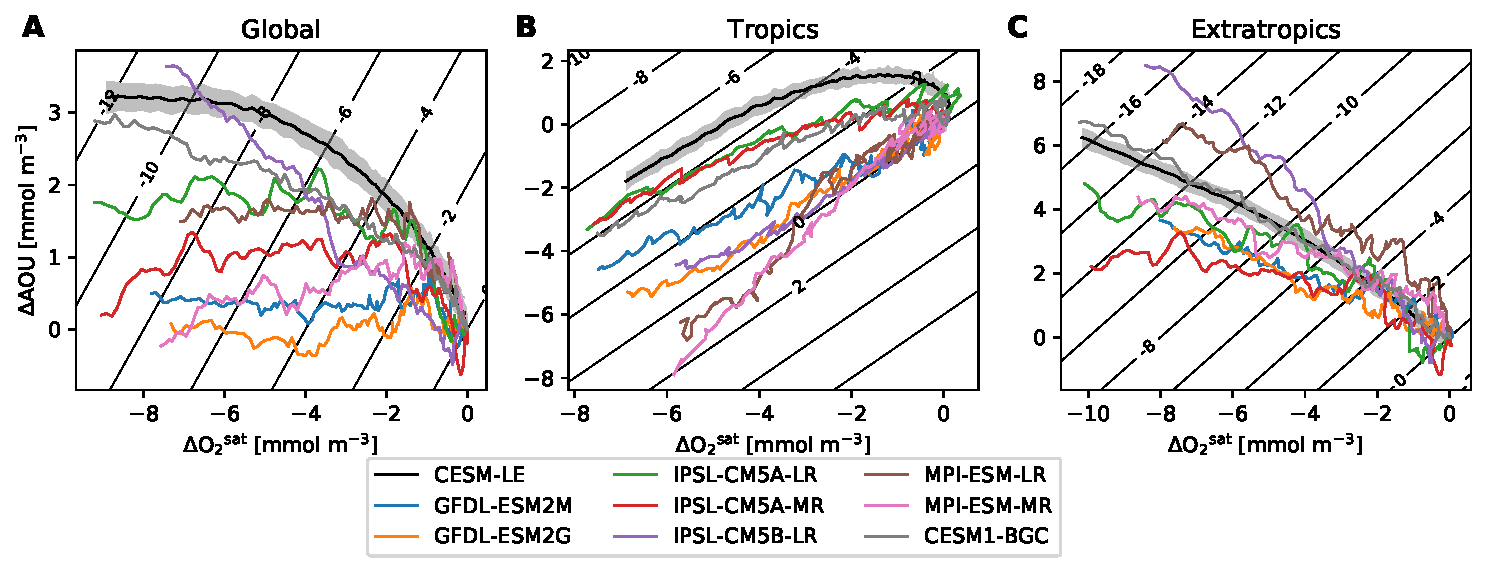
\includegraphics[width=1\textwidth]{aou-o2sat-phase-diag.pdf}
\caption{Simulated relationships between upper ocean (above 1000~m depth) ($\Delta{}AOU$) and $\Delta\ce{O2}^{sat}$ changes: (A) globally, (B) in the ``tropics'' (20$^\circ$S--20$^\circ$N), and (C) in the ``extratropics'' (poleward of 20$^\circ$ latitude).
The black line show results from the CESM-LE (shading shows the region within one standard deviation of the ensemble spread).
The colored lines show a subset of the CMIP5 models.
Contours show the total oxygen depletion.
}
\label{fig:aou-o2sat-phase}
\end{figure}
%-------------------------------------------------------------------------------

The divergent behavior within the CMIP5 models in the mechanisms driving upper ocean deoxygenation globally is partially a result of fundamentally different dynamics in the tropics versus high latitude regions; the models show more consistent behavior when these regions are considered separately (Figure~\ref{fig:aou-o2sat-phase}bc).
Deoxygenation in the extratropics (poleward of 20$^\circ$ latitude) is more intense than in the tropics and involves a combination of strong solubility and respiration effects; most models show trajectories near-perpendicular to the oxygen-change contours (Figure~\ref{fig:aou-o2sat-phase}c).
The CESM-LE simulates high latitude changes near the center of the CMIP5 model spread.
In contrast to $AOU$ increases in the extratropics, all CMIP5 models considered simulate decreasing $AOU$ in the upper ocean within the tropics (equatorward of 20$^\circ$ latitude; Figure~\ref{fig:aou-o2sat-phase}b).
Decreasing $AOU$ means less respiratory consumption of oxygen; therefore, while the models simulate warming-driven solubility declines in the tropics, reductions in $AOU$ compensate, tempering oxygen declines such that in some models, tropical oxygen is actually projected to increase by 2100 (Figure~\ref{fig:aou-o2sat-phase}b).
The CESM-LE is an end-member model in the simulation of tropical oxygen change; its initial trajectory includes modest oxygen decline driven by increased respiration (positive $\Delta{}AOU$); $AOU$ subsequently declines, however, at a rate that largely compensates for warming (Figure~\ref{fig:aou-o2sat-phase}b).
It is this initial reinforcing behavior in tropical and extratropical $AOU$ and subsequent cancelation that leads to the global trajectory for CESM-LE shown on Figure~\ref{fig:aou-o2sat-phase}a.

%-------------------------------------------------------------------------------
\begin{figure}[tbhp]
\centering
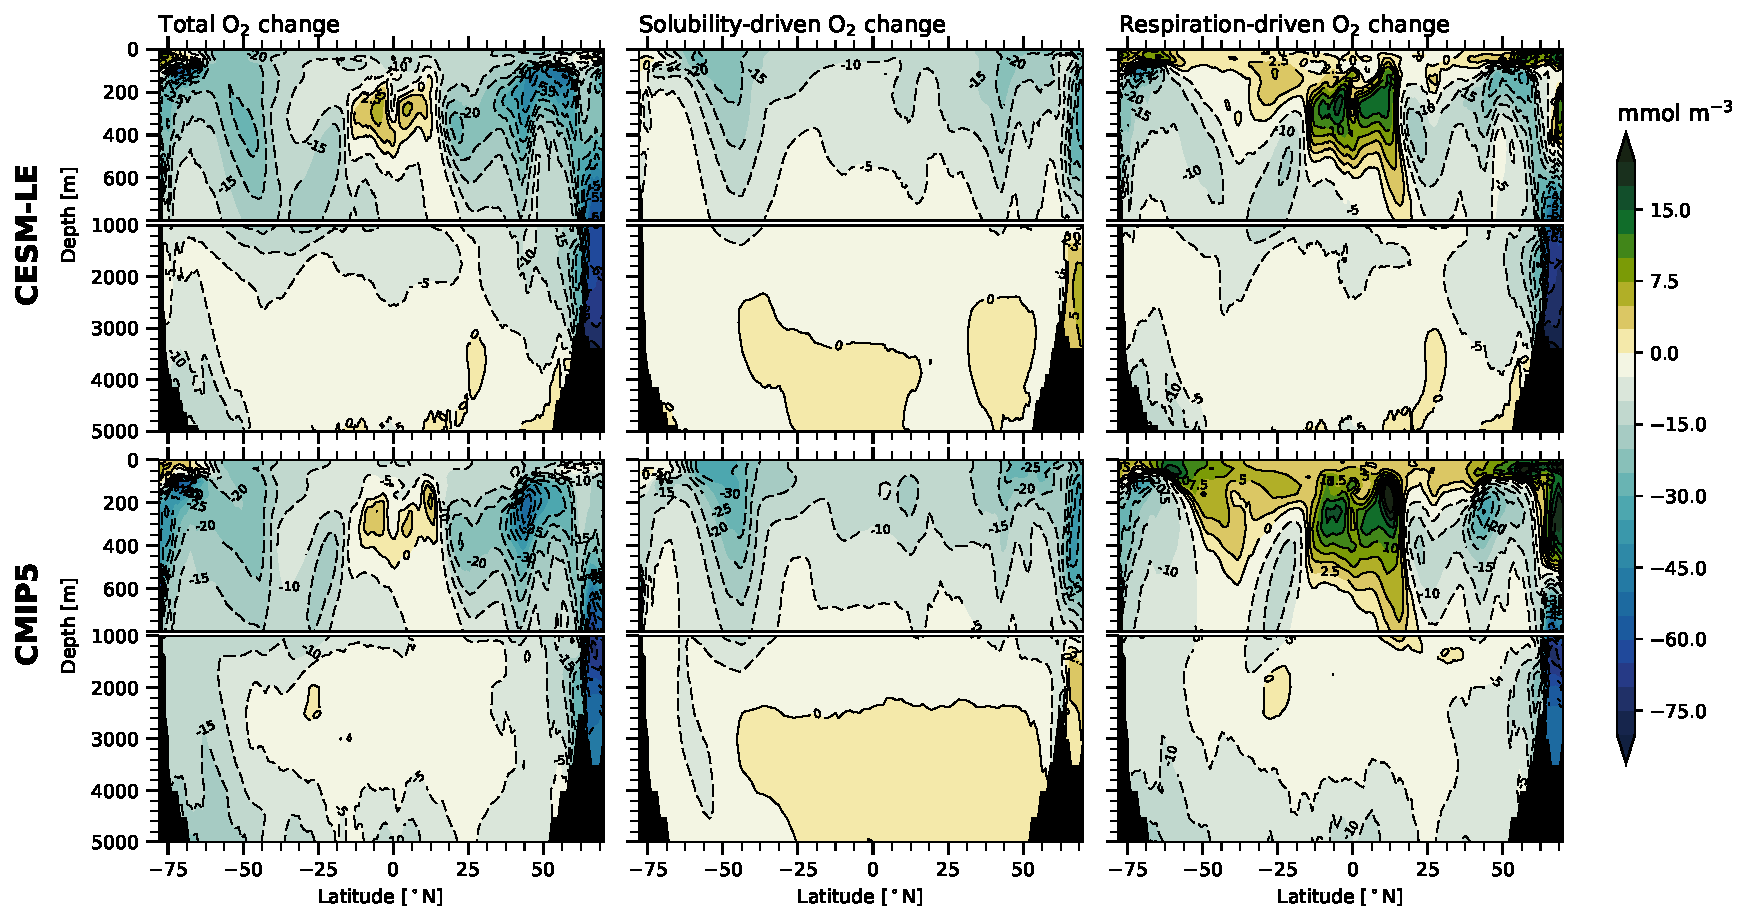
\includegraphics[width=1\textwidth]{global-zonal-mean-O2-AOU-O2sat.pdf}
\caption{Zonal-mean, ensemble-mean change in the concentration of dissolved oxygen in the ocean simulated by the (top row) Community Earth System Model Large Ensemble (CESM-LE) and the CMIP5 multi-model collection under RCP8.5.}
\label{fig:zonal-mean-section}
\end{figure}
%-------------------------------------------------------------------------------

Figure~\ref{fig:zonal-mean-section} shows the change in dissolved oxygen along a zonal-mean, depth section; the left column shows the total simulated oxygen change at 2100, while the middle and right columns shows the contribution of solubility and respiration to oxygen change.
This figure presents a picture consistent with that shown in Figure~\ref{fig:aou-o2sat-phase}: oxygen declines are most intense at high latitudes due to the reinforcing effects of solubility and respiration-driven change.
Opposing solubility and respiration effects mean that oxygen declines in the tropics are more modest---there is even a local oxygen increase in the low latitude thermocline.
The imprint of ocean ventilation pathways is evident on Figure~\ref{fig:zonal-mean-section} as regions of strong deoxygenation extending from surface to depth at mid-latitudes; these features are similar to those found in observations of oxygen declines \citep{Helm-Bindoff-etal-2011}.
Reductions in $AOU$ are evident at the surface globally (as we saw in Figure~\ref{fig:cesm-global-profile}), however, while the CMIP5 ensemble mean shows some weak $AOU$ declines in the extratropical southern hemisphere, the tropics are where pronounced $AOU$ declines above about 600~m depth compensate for solubility, leading to weak oxygen increases.

%-------------------------------------------------------------------------------
\begin{figure}[tbp]
\centering
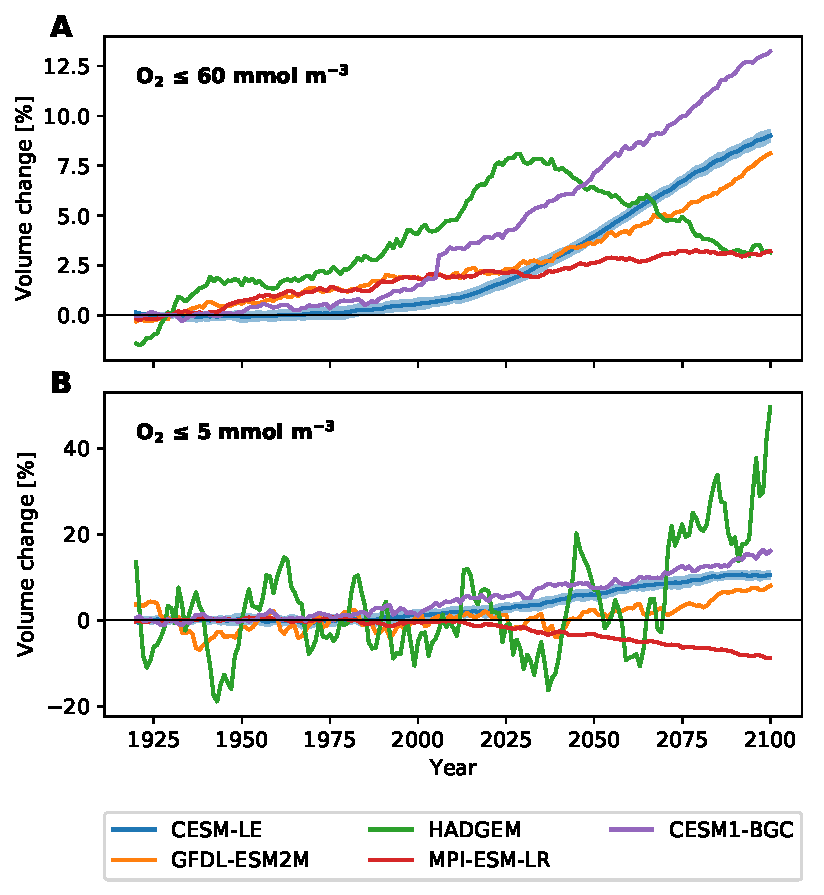
\includegraphics[width=0.6\textwidth]{volume-census.pdf}
\caption{Change in the volume of (A) hypoxic ($\ce{O2}\le60$~mmol~m$^{3}$) and (B) suboxic ($\ce{O2}\le5$~mmol~m$^{-3}$) waters in the CESM-LE (blue) and a subset of the CMIP5 models relative to a 1920--1939 baseline.
The CESM-LE has a average hypoxic volume of ${1.1\times10^{17}}$~m$^{3}$ over the period 1920--1939, whereas the CMIP5 ensemble mean hypoxic volume is ${9.2\times10^{16}}$~m$^{3}$.
The suboxic volumes are ${1.6\times10^{16}}$~m$^{3}$ and ${2.5\times10^{16}}$~m$^{3}$ for the CESM-LE and CMIP5 ensemble mean, respectively.
}
\label{fig:volumes}
\end{figure}
%-------------------------------------------------------------------------------

Figure~\ref{fig:volumes} shows the projected time-evolution of hypoxic ($\ce{O2}\le60$~mmol~m$^{-3}$) and suboxic ($\ce{O2}\le5$~mmol~m$^{-3}$) volumes in the CESM-LE and a subset of the CMIP5 ensemble.
All of the models show an increase in hypoxic volume by 2100, though hypoxic volume actually peaks mid-century in the HadGEM model.
Suboxic volume increases in all but one model, though the range of increase is large.
The coarse resolution of the ESMs precludes adequate representation of complex coastal processes; thus, these increases in hypoxic volumes do not properly reflect changes in coastal hypoxia.
They predominantly reflects changes to open-ocean regions in the tropics.

The distribution of \ce{O2} in the current ocean implies that suboxic zones are particularly sensitive to changes in regional oxygen concentrations.
A decline in mean \ce{O2} of the tropical upper ocean of only $\sim$2mmol~m$^{-3}$), substantially smaller than the global average,  is enough to double the current volume of suboxia globally \citep{Deutsch-Berelson-etal-2014}.
This expansion of suboxic zones would be associated with enhanced denitrification.
Assuming a constant volumetric rate of nitrogen loss in suboxic zones, integrated rates of denitrification would rise in proportion to the volume of suboxic waters, and may therefore also be exceptionally sensitive to deoxygenation.
Models of microbial nitrogen cycling in these regions indicate that the efficiency of nitrogen removal also increases as the volume of suboxic zones increases, so that the sensitivity of nitrogen loss to deoxygenation is further enhanced \citep{Penn-Weber-etal-2016}.
Historical reconstructions of nitrogen loss from the North Pacific based on sedimentary records and model hindcasts support a high sensitivity of denitrification, implying a 3-fold change in the integrated rate of denitrification in recent decades \citep{Deutsch-Berelson-etal-2014,Yang-Gruber-etal-2016}.
The impacts of historical changes in nitrogen loss can be seen in the nitrate deficit ($N^*$; see Figure~\ref{fig:o2pdfs} caption) well outside the suboxic zone, in the productive California Current System \citep{Deutsch-Brix-etal-2011}, with presumed impacts on the N-limited net primary production in that upwelling zone.
Large uncertainties still surround the future projections in the impacts of deoxygenation on nitrogen cycling and its effects on remote productivity.
Resolving these uncertainties will require models that better reproduce the mean state of the suboxic zones, the microbial dynamics in these regions, and the rates and pathways by which their nitrate deficits are transported to nitrogen limited surface regions, all of which are crudely represented in ESMs.

%-------------------------------------------------------------------------------
\subsection{Relationships with heat content}
%-------------------------------------------------------------------------------

We have just seen that deoxygenation is driven by the direct impact of temperature on solubility and the secondary effect of changes in circulation that lead to changes in respiration as estimated by $AOU$.
The CMIP5 models and the CESM-LE show that deoxygenation in the extratropics results from a synergy between these factors, which drive reinforcing changes in oxygen (Figure~\ref{fig:aou-o2sat-phase}c).
In the tropics, by contrast, the models suggest that solubility and respiration effects work in opposition; reductions in respiration tend to win-out slightly in some models, leading to modest increases in tropical oxygen (Figure~\ref{fig:aou-o2sat-phase}b).
While the models are relatively consistent with regard to these tendencies when the tropics and extratropics considered independently, divergent behavior results at the global scale due to averaging over regions with opposing tendencies.
Additionally, the opposing respiration-driven changes at high-latitude and in the tropics lead to cancelation, such that global deoxygenation in the multi-model mean is mostly solubility driven (Figure~\ref{fig:aou-o2sat-phase}a).
Another reason why the models might show different relative amounts of deoxygenation relates to the physical climate simulation: the models simulate different amounts of warming over the 21st century \citep{Bopp-Resplandy-etal-2013}.
This motivates us to consider the relationship between changes in oxygen with simulated changes in ocean heat content.

Figure~\ref{fig:o2-heat} shows the change in upper-ocean oxygen in each model plotted against the concomitant change in temperature; the top row of plots shows the period 1970--2014 and includes observational estimates; the bottom row shows 1970--2100.
Observational estimates of oxygen variability are from the data compilation of \citet{Ito-Minobe-etal-2017} and the ocean heat content estimates are from the European Centre for Medium-Range Weather Forecasts Ocean Reanalysis (ORAS4) \citep{Balmaseda-Trenberth-etal-2013}.
While the models were shown to have substantial differences in the mechanisms driving simulated oxygen decline, there is a fairly tight correspondence across the models between oxygen and temperature at the global scale (Figure~\ref{fig:o2-heat}ab); indeed, the relationship between the global mean \ce{O2} and global mean temperature above 1000~m depth tends to collapse into a quasi-linear relationship.
The dashed line in each panel of Figure~\ref{fig:o2-heat} shows the \ce{O2}-heat relationships that would arise if changes in \ce{O2} were purely solubility-driven.
Declines in \ce{O2} that exceed the solubility slope are due to the effect of respiration.

Notably, the observations indicate a much stronger \ce{O2}-heat relationship than is evident in any of the models.
Over recent decades, the global scale simulated \ce{O2}-heat relationship (Figure~\ref{fig:o2-heat}a) is in the range of $-7$ to $-13$~mmol~m$^{-3}$~K$^{-1}$; the observations, by contrast, show much more \ce{O2} loss for a given temperature increase, with a relationship of $-33.6\pm2.98$~mmol~m$^{-3}$~K$^{-1}$.
The observational estimates of \ce{O2}-heat relationships in the extratropics ($-32.2\pm2.47$~mmol~m$^{-3}$~K$^{-1}$; Figure~\ref{fig:o2-heat}e) and tropics ($-25.5\pm5.53$~mmol~m$^{-3}$~K$^{-1}$; Figure~\ref{fig:o2-heat}c) are also stronger than simulated.
The average slope of the simulated \ce{O2}-heat relationship is $-11.7$~mmol~m$^{-3}$~K$^{-1}$ in the extratropics, which is only slightly stronger than pure-solubility (Figure~\ref{fig:o2-heat}e), and the slope is very close to solubility ($-3.27$~mmol~m$^{-3}$~K$^{-1}$; Figure~\ref{fig:o2-heat}c) in the tropics.

Ocean warming between 1970 and 2014 is quite modest in comparison to the changes projected by 2100 (Figure~\ref{fig:o2-heat}ab).
Over the full 1970--2100 time period, the models show distinct behavior in the tropics and extratropics.
At the global scale and in the extratropics, deoxygenation is tightly coupled to temperature, with a slope that exceeds solubility in most models (Figure~\ref{fig:o2-heat}bf).
In the tropics, by contrast, all the models show less deoxygenation than would be predicted on the basis of solubility changes alone and the spread across the models in simulated oxygen change is wide (Figure~\ref{fig:o2-heat}d).
Tropical oxygen loss in the CESM-LE, for instance, begins with a temperature relationship much stronger than solubility, but the rate of decline with respect to temperature diminishes, ultimately yielding a relationship integrated out to 2100 that is less than would be predicted from pure solubility-driven changes (Figure~\ref{fig:o2-heat}d).

It is not clear what causes these large differences in the sensitivity of ocean oxygen content to the heat uptake.
The observations themselves involve substantial uncertainty, much of which arises from the fact that oxygen measurements are relatively sparse in space and time---and particularly sparse in the tropics.
Furthermore, as we lack long-term records of oxygen trends on the global scale, it is possible that the observations include periods or regions strongly influenced by natural variability, which may involve a different mix of solubility and respiratory ($AOU$) changes.
It is also possible that the models are missing a mechanism that is actually driving \ce{O2} declines in nature.
For instance, \citet{Ito-Nenes-etal-2016} showed that polluted aerosol deposition has driven substantial declines in tropical Pacific oxygen concentration over recent decades.
If ESMs lack such forcing, which may be strongly correlated temporally with ocean heat content, they should predict an \ce{O2}-temperature relationship that is too weak.
Similarly, the models may omit important changes due to ocean acidification, stoichiometry and specifics of tropical wind forcing \citep[][and references therein]{Oschlies-Duteil-etal-2017}.

In summary, the collection of CMIP5 models and the CESM-LE are relatively consistent in their simulation of \ce{O2}-heat relationships in the extratropics; however, there is little agreement on this relationship in simulations of the tropics.
Observations indicate a stronger \ce{O2}-heat relationship than is simulated by any of the models, which suggests that the models underestimate the amount of respiration-driven deoxygenation.
If we believe that the observations provide an accurate assessment of the true \ce{O2}-heat relationship, the implication is that the simulated deoxygenation is a substantial underestimate of the oxygen loss that will be realized for a given warming scenario.

%-------------------------------------------------------------------------------
\begin{figure}[tbp]
\centering
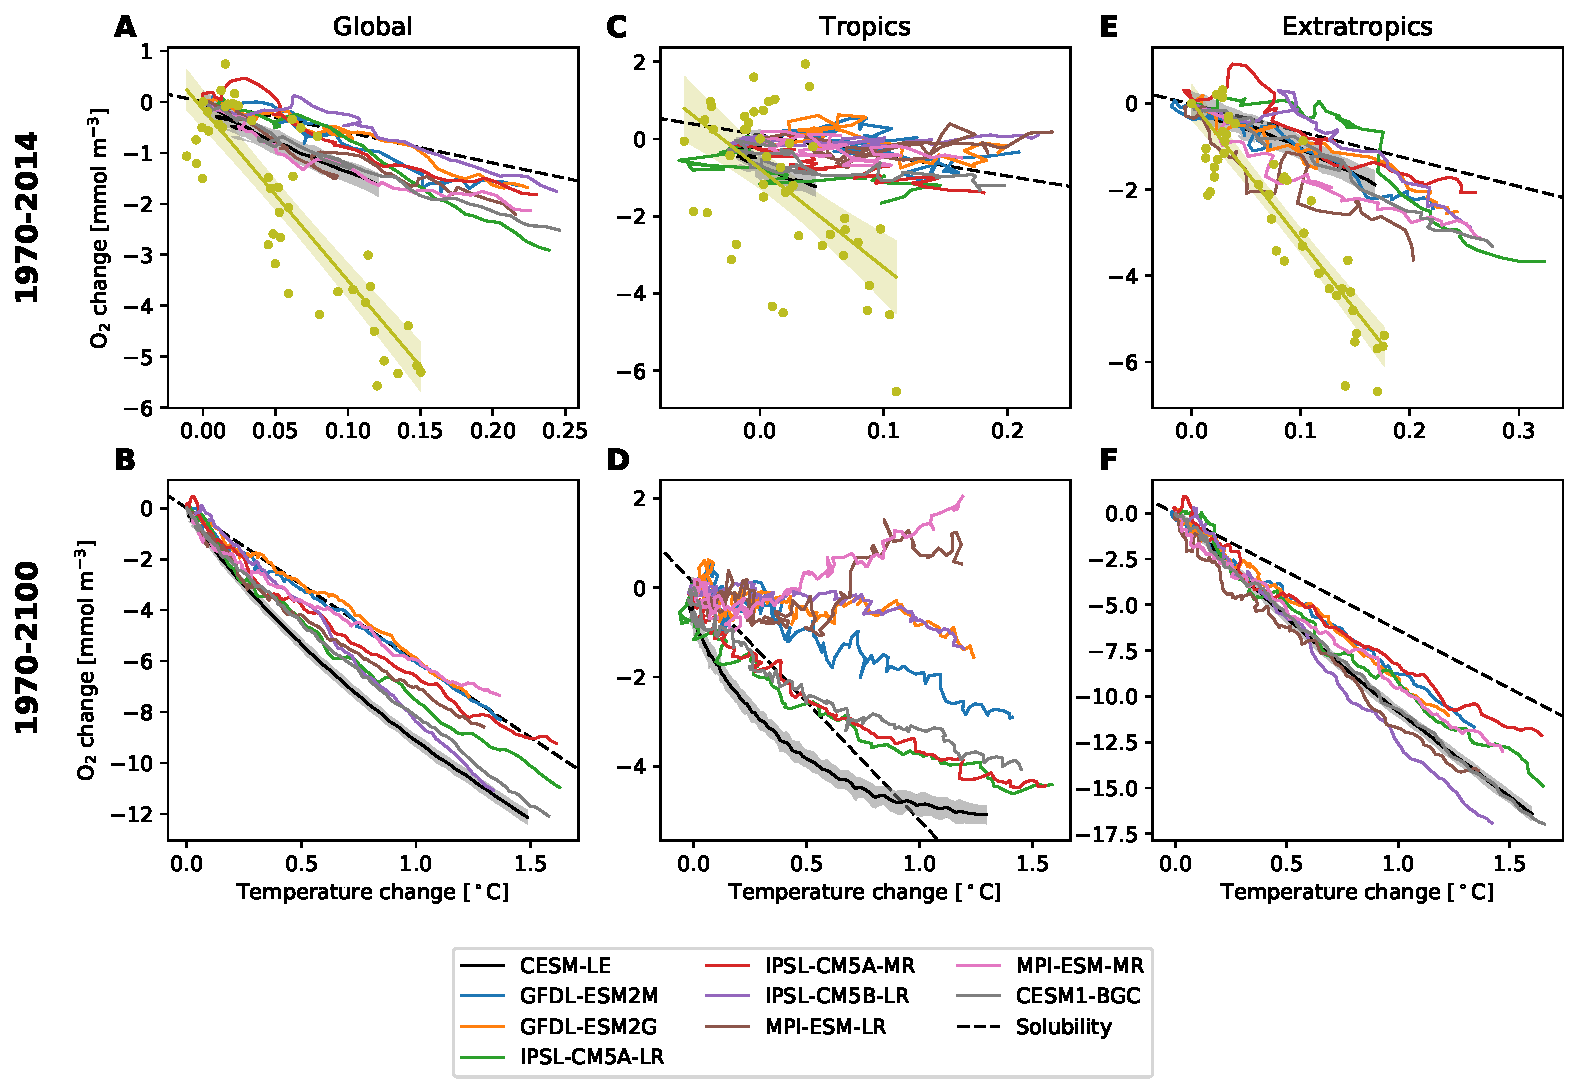
\includegraphics[width=1.1\textwidth]{o2change-temp-phase-diag.pdf}
\caption{Modeled and simulated relationships between upper ocean (above 1000~m depth) mean \ce{O2} and temperature changes.
Top row shows model and observational data over the period 1970--2014; the bottom row shows the models from 1970--2100; annual means are plotted and all change is relative to the year 1970.
The left column shows data averaged globally; the middle column shows data averaged in the tropics (20$^\circ$S--20$^\circ$N); and the right column shows  the extratropics (poleward of 20$^\circ$ latitude).
Simulation data is taken from a subset of the CMIP5 models (noted in legend) and the CESM-LE.
Observational data is taken from \citet{Ito-Minobe-etal-2017}.
The dashed line in the each panel indicates the expected relationship if all change in oxygen was solubility-driven.
}
\label{fig:o2-heat}
\end{figure}
%-------------------------------------------------------------------------------

%-------------------------------------------------------------------------------
\subsection{Oxygen change in the thermocline}
%-------------------------------------------------------------------------------

While the global trends in oxygen are characterized by consistent secular declines (Figure~\ref{fig:cesm-global-timeseries}), regional patterns of change, as we have just seen, are more complicated; thus, we next examine patterns in oxygen over the thermocline, which we take to be over the 200--600~m depth range.
Our focus on the thermocline depth is motivated by relevance to ecological impacts.
As the base of the oxygenated surface layer, oxygen declines in this depth range might drive vertical habitat compression, impacting marine organisms that are concentrated in the near surface \citep{Stramma-Prince-etal-2011,Deutsch-Ferrel-etal-2015}.

%-------------------------------------------------------------------------------
\begin{figure}[tbp]
\centering
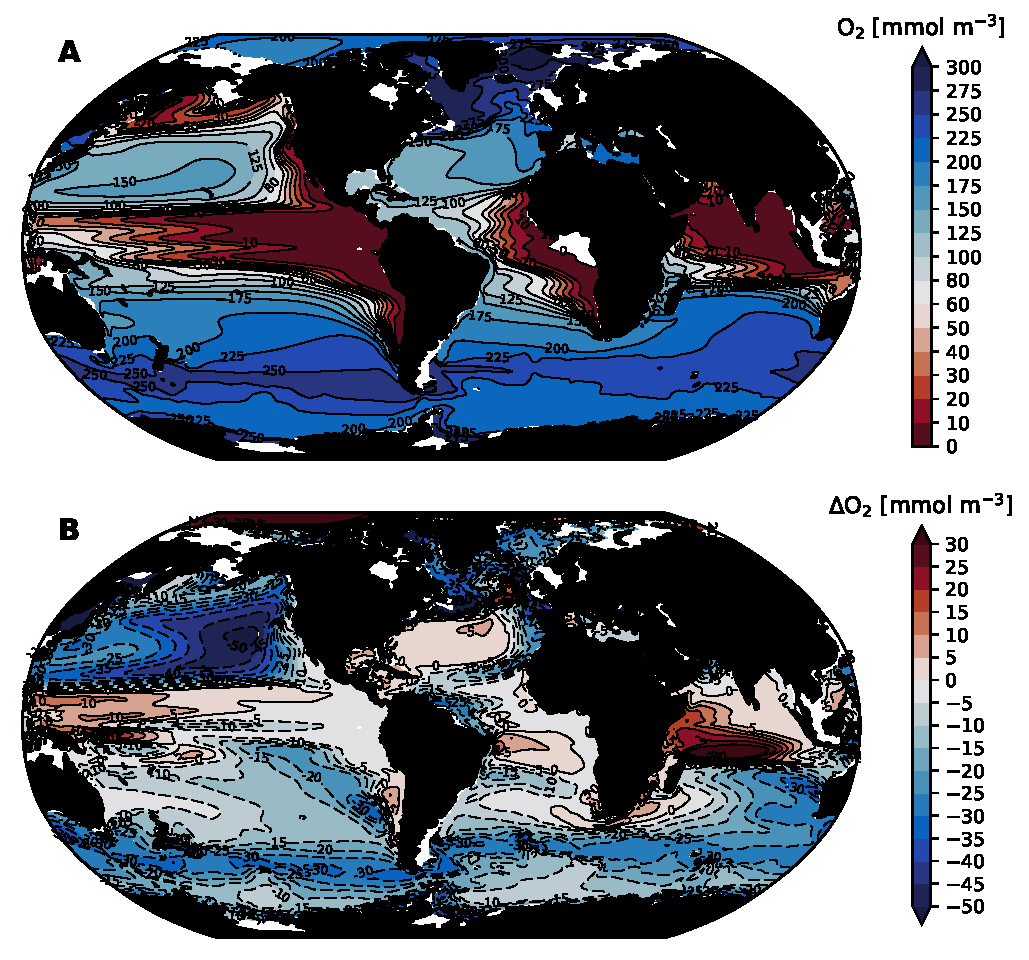
\includegraphics[width=0.8\textwidth]{cesm-thermocline-o2-change.pdf}
\caption{Thermocline (mean over the 200--600~m depth range) oxygen distributions simulated by the CESM-LE: (A) \ce{O2} concentration in the control climate; (B) change in \ce{O2} concentration at 2100.
We use the ensemble mean over the period 1920--1939 to define the ``control'' climate.}
\label{fig:cesm-thermocline-o2-change}
\end{figure}
%-------------------------------------------------------------------------------

Figure~\ref{fig:cesm-thermocline-o2-change}a shows the distribution of oxygen in the ``control'' climate of the CESM-LE.
It is important to note the discrepancies between this simulated oxygen distribution and that inferred from observations (Figure~\ref{fig:woa-thermocline-o2-age}a): oxygen concentrations in CESM-LE tend to be too low and hypoxic regions are too extensive.
These biases, a well-known and common feature of coarse-resolution ESMs, are partially attributable to sluggish circulation yielding weak ventilation and are discussed further in section~\ref{loc:structural-uncertainty}.
In spite of the biases in simulated oxygen distributions, however, the basic spatial structure of the oxygen field is well represented (i.e., the pattern correlation with observations is relatively high); thus, we are confident that this model (and other ESMs) can provide some insight into the mechanisms driving deoxygenation---though projections for oxygen variability and trends in tropical OMZs are to be treated with particular caution.

Thermocline oxygen depletion at 2100 is most pronounced in extratropical regions, with particularly strong changes in the North Pacific (Figure~\ref{fig:woa-thermocline-o2-age}b).
Consistent with what we have already seen, there are modest increases in oxygen in the tropics in all ocean basins, with moderately strong increases in the western equatorial Pacific and Indian Oceans.
In order to understand the mechanisms modulating the intensity of deoxygenation and its spatial structure, it is instructive, once again, to examine the direct temperature effects on oxygen decline ($\Delta\ce{O2}^{sat}$) and respiration-driven declines ($\Delta{}AOU$).
These fields are shown in Figure~\ref{fig:cesm-thermocline-o2sat-aou-change}, noting that, as in Figure~\ref{fig:cesm-global-profile}, we plot the negative of the $\Delta{}AOU$, which can be directly interpreted as the change in oxygen due to changes in respiration, presuming that surface waters remain close to  equilibrium with atmospheric \ce{O2}.
The structure in $\Delta\ce{O2}^{sat}$ is a direct reflection of changes in ocean temperature in the thermocline depth range; $\Delta\ce{O2}^{sat}$ is strongly negative in the Southern Ocean, the Arctic, and parts of the North Atlantic.
The Southern Ocean dominates ocean heat uptake in the present-day climate \citep{Talley-Feely-etal-2015} and is expected to persist in this role under future warming scenarios \citep{Frolicher-Sarmiento-etal-2015}.
The North Atlantic, as a site of substantial deepwater formation, also plays a strong role in ocean heat uptake; however, the patterns associated with the ``warming hole'' lead to localized cooling where solubility-driven changes in oxygen are positive (Figure~\ref{fig:cesm-thermocline-o2sat-aou-change}a).
There is no substantial deepwater formation in the Arctic basin; however, this region is subject to strong sea ice declines and warming associated with polar amplification \citep{Screen-Simmonds-2010} leading to widespread reductions in solubility in this region.

%-------------------------------------------------------------------------------
\begin{figure}[tbp]
\centering
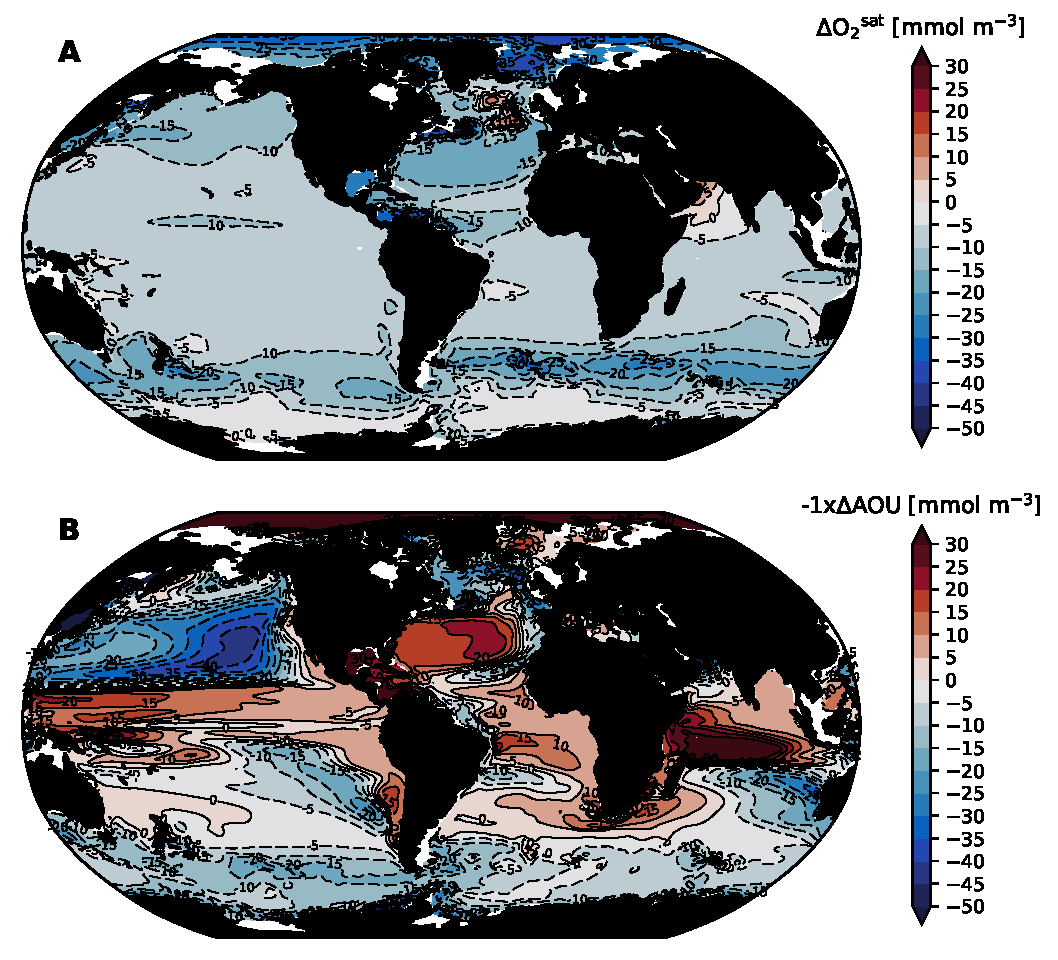
\includegraphics[width=0.8\textwidth]{cesm-thermocline-o2-change-sat-aou.pdf}
\caption{Solubility and respiration-driven changes in thermocline (200--600~m mean) oxygen at the year 2100; computed from the CESM-LE ensemble mean:
(A) Solubility-driven oxygen change ($\Delta\ce{O2}^{sat}$).
(B) Respiration-driven oxygen change (the negative of $\Delta{}AOU$).}
\label{fig:cesm-thermocline-o2sat-aou-change}
\end{figure}
%-------------------------------------------------------------------------------

While the direct effect of temperature on oxygen is almost universally negative (driving declines), changes associated with respiration are more complicated (Figure~\ref{fig:cesm-thermocline-o2sat-aou-change}b).
By examining the changes in $AOU$, we can see that strong oxygen depletion in the thermocline of the North Pacific is a result of increases in respiration-driven oxygen depletion (increased $AOU$) that reinforce temperature effects.
This contrasts with the North Atlantic, where respiration-driven declines in oxygen (increased $AOU$) are confined to the subpolar gyre; $AOU$ in the mid-latitude North Atlantic thermocline decreases, which mitigates solubility driven oxygen declines there.
Tropical regions are characterized by widespread declines in $AOU$, indicative of reduced oxygen consumption by respiration, consistent with the picture gleaned from our analysis of the $\Delta AOU$-$\Delta\ce{O2}^{sat}$ phase space for the tropics (Figure~\ref{fig:aou-o2sat-phase}b).

%-------------------------------------------------------------------------------
\begin{figure}[tbp]
\centering
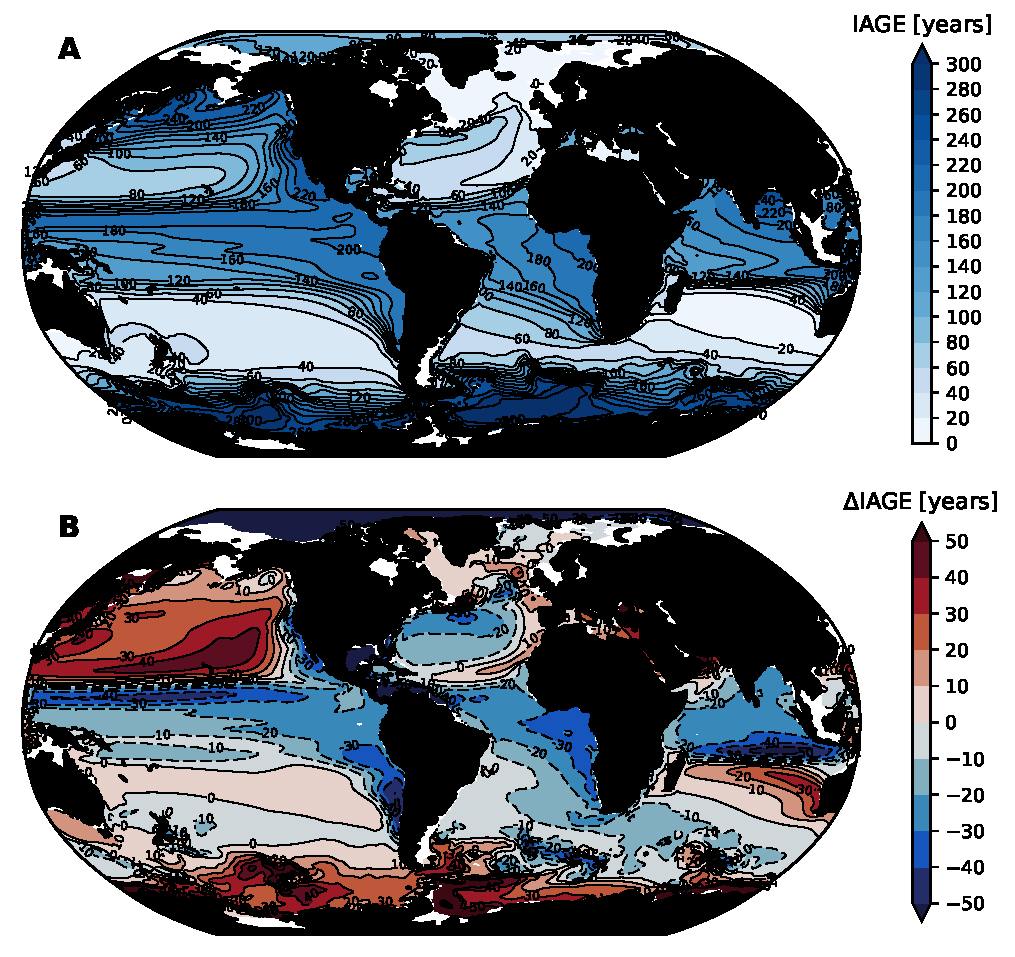
\includegraphics[width=0.8\textwidth]{cesm-thermocline-iage-change.pdf}
\caption{Thermocline (mean over the 200--600~m depth range) ideal age (IAGE) distributions simulated by the CESM-LE: (A) IAGE in the control climate; (B) change in IAGE at 2100.}
\label{fig:cesm-thermocline-iage-change}
\end{figure}
%-------------------------------------------------------------------------------

Why are there decreases in cumulative respiration ($AOU$) in the tropical thermocline under climate warming?
Our first clue to answering this question come from looking at the distibution of water mass age in the CESM-LE simulation. Figure~\ref{fig:cesm-thermocline-iage-change} shows the mean distribution and change in a tracer called ``ideal age'' (IAGE) in the CESM-LE.
Ideal age is transported by the OGCM; it is set to zero in the surface layer and increases at a rate of 1 year per year in the ocean interior---thus providing a direct estimate of the average time since a water-mass was last in contact with the atmosphere.
Just as we saw in section~\ref{loc:o2-distributions}, there is a tight correspondence between the age of waters in the thermocline (Figure~\ref{fig:cesm-thermocline-iage-change}a) and their oxygen content (Figure~\ref{fig:cesm-thermocline-o2-change}a); older waters tend to have lower \ce{O2} concentrations.
Similarly, the change in the age of thermocline waters at 2100 is a relatively good predictor of changes in oxygen; waters that become older show \ce{O2} declines, whereas waters that become younger have modest increases in oxygen.
As discussed above, water mass age controls $AOU$ by determining the time available for a respiration signal to accumulate.
If we imagine the flow in the ocean interior as consisting of a one-dimensional pipe, a reduction in age is akin to moving upstream in that pipe, where water mass properties are closer to those of the inlet at the ocean surface.
The reduction in ideal age with the tropical thermocline is likely due to a shift in the relative balance of water masses contributing to these regions \citep{Gnanadesikan-Russell-etal-2007}.
In particular, as upwelling in the tropics is diminished under climate warming, the contribution of old deep waters to the thermocline is reduced, leading to a local reduction in age.

Another mechanisms that might lead to local increases in oxygen is a reduction in $OUR$; indeed, changes in $AOU$ can be thought of as originating from changes in age and/or changes in $OUR$.
As we noted in section~\ref{loc:o2-distributions}, net primary productivity in the surface ocean is expected to decline under climate warming, which will drive diminished export of organic matter, thereby alleviating the demand for oxygen in ocean interior.
Most of the CMIP5 models do indeed simulate declines in net primary productivity under climate warming, though there is substantial differences between the models and some simulate an increase \citep{Laufkotter-Vogt-etal-2015}.
A reduction of $OUR$ was found to be the dominant mechanism driving multi-decadal changes in suboxic zone volume and denitrification in retrospective model simulations of the tropical Pacific that reproduce observed changes in nitrogen cycle tracers \citep{Deutsch-Brix-etal-2011,Deutsch-Berelson-etal-2014}.
Figure~\ref{fig:cesm-carbon-export} shows the change in carbon export in the CESM-LE.
There is a global reduction in export production, with the strongest reductions in the North Atlantic; export production increases, however, over broad regions of the Southern Ocean and tropical Pacific.
The widespread reduction in export production in the North Atlantic might be expected to temper oxygen declines in that basin, consistent with the reduction in $AOU$ (Figure~\ref{fig:cesm-thermocline-o2-change}b).
The changes in $OUR$ in the tropical Pacific, however, are more complicated and further analysis is necessary to assess the role of changes in $OUR$ in driving oxygen change there.

%-------------------------------------------------------------------------------
\begin{figure}[tbp]
\centering
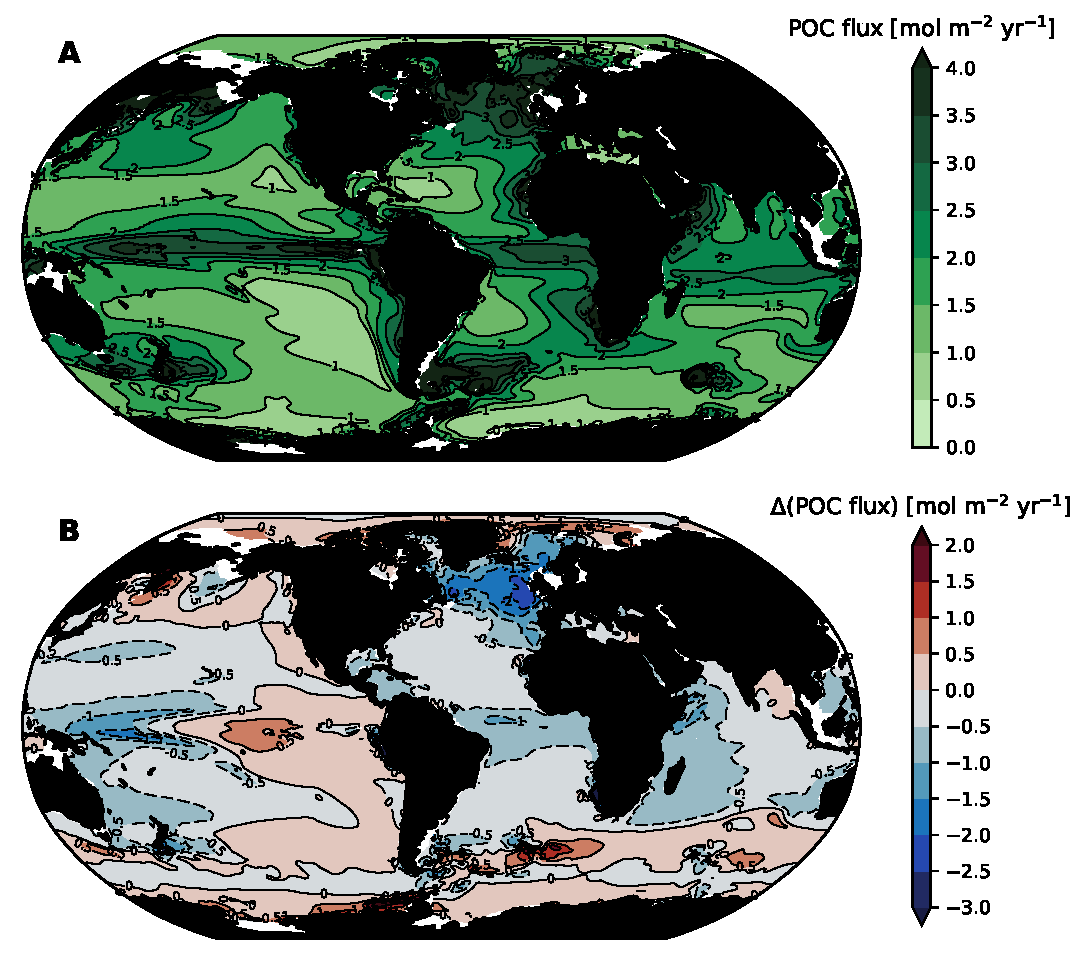
\includegraphics[width=0.8\textwidth]{cesm-export-production.pdf}
\caption{Carbon export at 100~m in the CESM-LE.}
\label{fig:cesm-carbon-export}
\end{figure}
%-------------------------------------------------------------------------------

%-------------------------------------------------------------------------------
\subsection{Time of emergence}\label{loc:toe}
%-------------------------------------------------------------------------------

One question that arises in the context of interpreting observations is whether trends are attributable to human-driven climate change.
A key challenge in making definitive assessments of attribution is the role of natural climate variability, which has the potential to drive long-term trends in ocean oxygen.
Indeed, variations in weather from year-to-year can produced thermally-driven surface \ce{O2} anomalies, modulate surface-to-depth exchange, and alter the structure of the upper ocean environment, thereby impacting organic matter production and $OUR$ in the interior \citep{Ito-Deutsch-2010,Deutsch-Brix-etal-2011}.
Observations collected in the Labrador Sea, for instance, have linked regional variations in \ce{O2} to changes in deep convection on decadal or shorter timescales \citep{van-Aken-Femke-de-Jong-etal-2011}.
In the subpolar North Pacific, oxygen  displays significant variability \citep{Deutsch-Emerson-etal-2006}, which has been linked to fluctuations in the winter-time atmospheric forcing of the ocean \citep{Andreev-Baturina-2006}.
Variability of thermocline \ce{O2} ventilation in the North Pacific is mainly controlled by the areal extent of winter mixed layer water intersecting the density layers through which atmospheric \ce{O2} is supplied to the ocean \citep{Kwon-Deutsch-etal-2016}.


%-------------------------------------------------------------------------------
\begin{figure}[tbp]
\centering
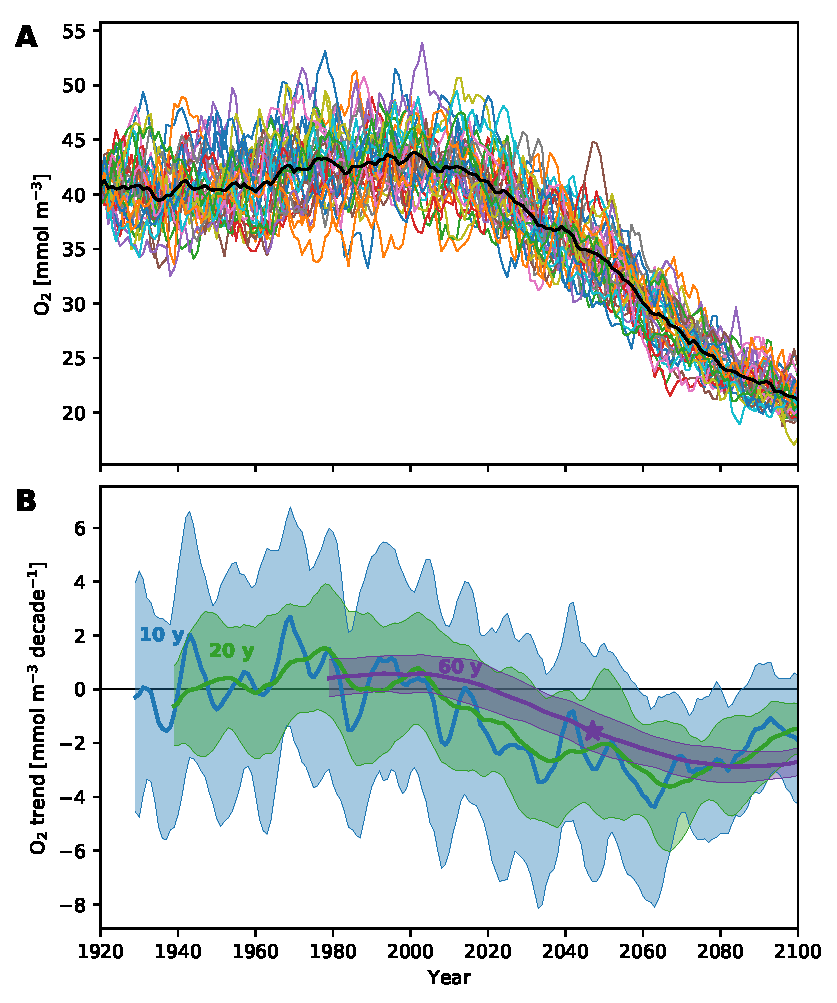
\includegraphics[width=0.8\textwidth]{cesm-regional-ccs-timeseries.pdf}
% generated by: plot_cesm_zonal_sections.ipynb
\caption{Oxygen concentrations and trends in the thermocline of the California Current System (CCS) simulated by the CESM-LE.
(A) Oxygen concentrations in the CCS; colored lines show individual ensemble members; black line is the ensemble mean.
(B) Retrospective trends computed from the data displayed in panel (A).}
\label{fig:ccs}
\end{figure}
%-------------------------------------------------------------------------------

Our view of global-scale changes in ocean oxygen leaves an impression of smooth changes and clear trends (Figure~\ref{fig:cesm-global-timeseries}a).
Indeed, at the global-scale, spatial averaging reduces the contribution of natural variability to fluctuations in oxygen concentrations, which is reflected in relatively little ensemble spread.
The case is different moving to regional scales; here, natural variability crops up as major driver of trends.
Figure~\ref{fig:ccs}a, for instance, shows oxygen concentrations simulated by the CESM-LE in thermocline depth range in the California Current System (CCS; 33--46$^\circ$N, within $\sim$800~km of the coast).
Notably, there is substantial variability in oxygen at this regional scale.
Each colored line in Figure~\ref{fig:ccs}a shows the oxygen concentration in the CCS for a particular ensemble member; these lines can each be considered equally plausible realizations of the historical period.
There is substantial spread because the timing of modes of natural climate variability are out of phase across the ensemble; the fluctuations amount to weather-like noise and are entirely natural.
Changes driven by increasing greenhouse gas concentrations, however, are superimposed on the natural variability; this ``forced'' signal is evident most clearly in the ensemble mean.
Just as spatial averaging to the global-scale decreases noise, averaging across the ensemble tends to cancel out the effects of natural variability, leaving only the forced signal.

Given the role of natural variability in driving random fluctuation, detection and attribution of human-driven climate change amounts to a signal-to-noise problem.
For detection to be possible, forced signals must develop magnitude and persistence sufficient to transcend the noise, which is characterized by the envelop of background variability \citep{Hasselmann-1993,Santer-Bruggemann-etal-1994,Santer-Mears-etal-2011}.
In this context, internally-generated variability inherently limits detection of climate-change signals regardless of practical observing capabilities; inferring trends from sparse observations is an obvious additional complication.

To illustrate the issues associated with detection and attribution of human-forced climate change, we consider the ``time of emergence'' (ToE) of the forced signal in the CCS region.
We use a relatively narrow definition of ToE, in which we compare the magnitude of trends in oxygen to the variability of similar trends across the ensemble.
We compute retrospective trends in each ensemble member starting at the year 2000 and continuing through the year 2100.
For each year, we compute trends over record lengths from 10 to 100 years.
We normalize the trends computed at each year and record length by the standard deviation of trends within the full CESM-LE, yielding a signal-to-noise ratio estimate.
We then diagnose ToE as the earliest year in which a trend of any length is more than two standard deviations ($2\sigma$) outside the variability in trends across the ensemble and does not return to within $2\sigma$ for all remaining years in the simulation.

The results of this computation for thermocline oxygen in the CCS are illustrated in Figure~\ref{fig:ccs}b.
Each line shows the ensemble mean trend and the shaded region shows the range within one standard deviation of the mean; blue shows 10 year trends, green shows 20 year trends and purple shows 60 year trends.
As is evident from the 10 year trends, there is substantial decadal variability in oxygen in the CCS within the CESM-LE simulation; trends span a wide range from strongly increasing to strongly decreasing \ce{O2}.
As the trend length moves to 20 years in duration, the spread across the ensemble is diminished and the variability in the ensemble mean trend is reduced.
However, even with 20 year trends, it is not possible to identify a ToE for forced \ce{O2} change in the CCS in this simulation---even out to 2100.
Trends of 60 years in length further reduce the noise, however, and detection of anomalous trends is possible around 2050 (the purple star).

%-------------------------------------------------------------------------------
\begin{figure}[tbp]
\centering
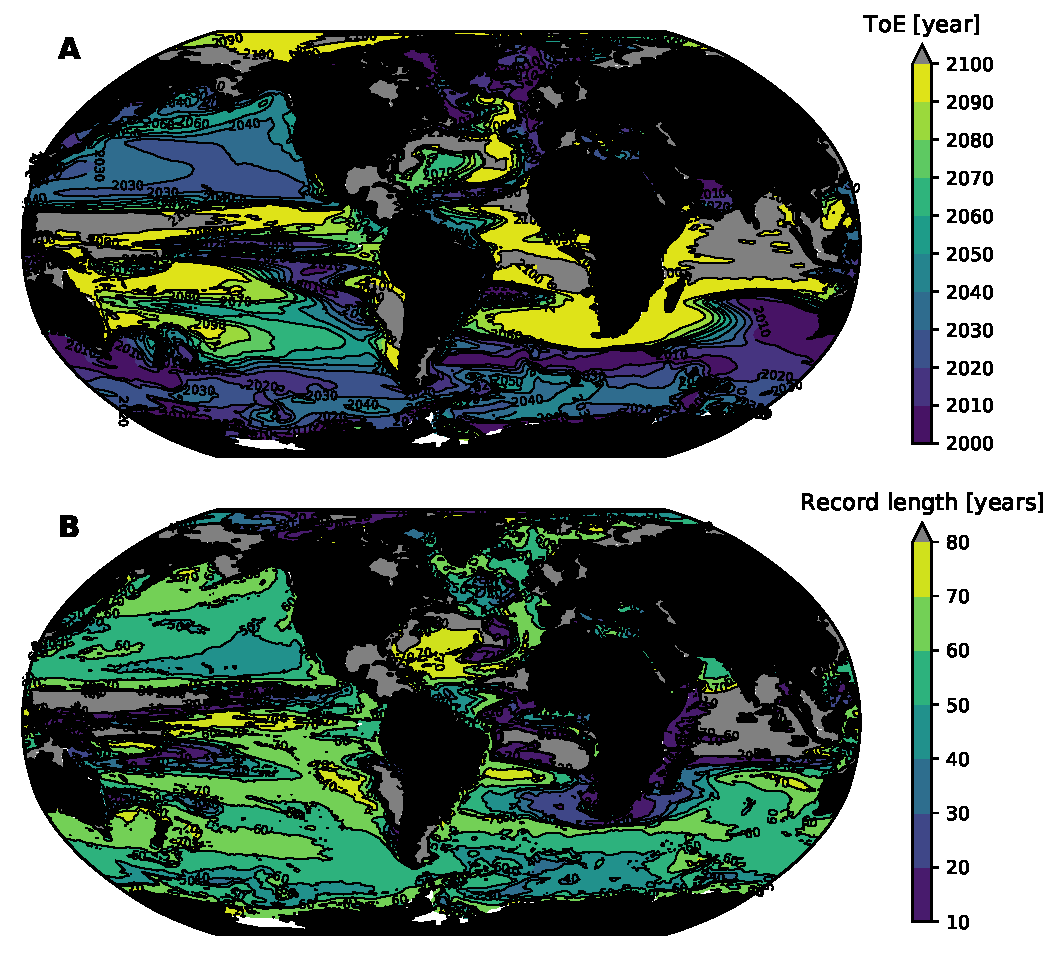
\includegraphics[width=0.8\textwidth]{cesm-toe.pdf}
% generated by: plot_cesm_zonal_sections.ipynb
\caption{Time of emergence for trends in thermocline (mean over the 200--600~m depth range) oxygen, as simulated by the CESM-LE: (A) the year at which a significant trend is detected on average across the ensemble; and (B) the length of record required to detect a significant trend.
Gray areas are regions where detection was not possible by 2100; in some cases these are regions where oxygen increased.}
\label{fig:cesm-toe}
\end{figure}
%-------------------------------------------------------------------------------

Figure~\ref{fig:cesm-toe} shows the results of this same computation applied to thermocline oxygen globally.
Interestingly, while the North Pacific has some of the strongest deoxygenation signals at 2100 (Figure~\ref{fig:cesm-thermocline-o2-change}), the detection of ToE on the basis of trends in this region is delayed until the 2030s and 2040s.
Broad region of the Southern Ocean and high latitude North Atlantic, by contrast, show relatively advanced detection times: in the early 2000s.
Figure~\ref{fig:cesm-toe}b illustrates, however, that detection of the forced signal can require fairly long observational records.
Indeed, over much of the areas where early detection is possible, identifying ToE requires records of 40--60 years in length.

In addition to trends, there are other elements of the time-evolving signal-to-noise relationship that can facilitate identifying ToE \citep{Santer-Bruggemann-etal-1994}.
First, changes in the mean value of dissolved oxygen concentrations may be compared to the variability over a period known to have little influence from external forcing.
In this context, as concentrations pass outside the range of unforced variability, these changes might be classified as externally forced \citep{Christian-2014}.
Second, the large-scale spatial structure associated with the forced signal can be evaluated relative to the dominant spatial structures associated with natural oxygen variability.
Detection in this context relies on the extent to which the pattern associated with a forced signal is distinct from the patterns associated with natural variability.
We considered these methods in \citet{Long-Deutsch-etal-2016}; a key point from all approaches is that high quality, sustained observing systems are critical to enabling early detection.

This discussion is not meant to cast doubt on the notion that the ocean is losing oxygen due to anthropogenic forcing.
Rather, it is important to emphasize that natural climate variability can make substantial contributions to oxygen trends at local to regional scales---and this must be considered in the interpretation of observations.
It is scientifically useful to understand the mechanisms driving \ce{O2} fluctuations, and ideally be able to attribute variability to natural versus human-driven causes.
Ultimately, with sufficient investments in observing and modeling capabilities, it may be possible to forecast large-scale oxygen anomalies years in advance.
Improvements in our understanding of oxygen variability and trends could reduce uncertainty in the nature, magnitude, and impact of climate change on marine ecosystems, thereby providing a more reliable basis for adaptation strategies and understanding cost/benefit trade-offs associated with climate change mitigation.

%-------------------------------------------------------------------------------
\section{Implications and uncertainties}
%-------------------------------------------------------------------------------

Our focus in this chapter thus far has been to describe how large-scale oxygen distributions are expected to change.
We have relied on ESMs because these provide a comprehensive basis for assessing interactions between climate and ocean biogeochemistry under future forcing scenarios.
As has been alluded to many times above, however, ESMs are far from perfect; their deficiencies merit additional attention, which we will apply here, with a focus on characterizing the structural uncertainty in model projections.
In addition to uncertainty, there are several implications of deoxygenation that are not directly simulated by the ESMs discussed above.
These include the impacts on \ce{N2O} production as a result of hypoxic and suboxic zone expansion.
Additionally, the deoxygenation problem is likely to manifest at spatial scales smaller than those easily amenable to study with global ESMs.
In particular, it is very likely that coastal marine systems will be impacted by ocean deoxygenation, so we include some discussion of this below.
Finally, our ability to understand how the structure and function of ecosystems will change in response to deoxygenation is a major challenge.
We discuss an approach to characterizing the projected future environmental change directly in ecophysiological terms.

%-------------------------------------------------------------------------------
\subsection{Structural uncertainty} \label{loc:structural-uncertainty}
%-------------------------------------------------------------------------------

The ESM projections discussed above suggest that the ocean will lose substantial oxygen over the 21st century.
Deoxygenation will be most intense at high latitudes due to the combined effects of solubility and respiration-driven reductions.
Oxygen loss in the tropics is more ambiguous; the models project modest increases in oxygen within the tropical thermocline, where declines in solubility are offset by declines in respiration that are largely driven by changes in circulation (Figure~\ref{fig:zonal-mean-section}).
Most models show an increase in hypoxic and suboxic volumes, indicating that while the intensity of oxygen depletion in the core of oxygen minimum zones is diminished, these zones will expand in future.
However, while the models provide a relatively consistent picture in their projections of high latitude deoxygenation, there is limited consensus on the balance of mechanisms driving projected tropical oxygen change (i.e., Figures~\ref{fig:aou-o2sat-phase}b and \ref{fig:o2-heat}b).
We will discuss the implications of this uncertainty in this section and attempt to provide perspective on why models solutions might be biased.

First, it is well recognized that the state-of-the-art ESMs struggle to accurately reproduce the observed mean state of oxygen distributions and biases are most pronounced in the tropics, where oxygen levels are very low \citep{Bopp-Resplandy-etal-2013}.
Common biases are characterized by oxygen distributions that are generally too low and oxygen minimum zones that are (vastly) too extensive, though not all models have this combination of biases \citep{Bopp-Resplandy-etal-2013}.
The distribution of very low oxygen involves a subtle interplay of physical and biological mechanisms; getting the balance of these correct is clearly challenging.
For instance, the derivative of the oxygen solubility relation with respect to temperature (Figure~\ref{fig:o2-sol}) is approximately $-5$~mmol~m$^{-3}$ per degree.
This suggests that a 1$^\circ$C bias in sea surface temperatures can make a substantial difference in downstream waters near the suboxic threshold of 5~mmol~m$^{-3}$.

ESMs are also limited by their relatively coarse spatial resolution, which is constrained by computational cost.
Ocean dynamics are characterized by motions on scales ranging from sub-meter to planetary; most of the kinetic energy in the ocean in contained within currents that have spatial scales ranging from 10 to 100~km; this range of spatial scales is defined as the ocean mesoscale \citep{Stammer-1997}.
The resolution of the OGCMs used by ESM is too coarse to explicitly represent mesocale dynamics; thus, these motions must be approximated with subgrid-scale parameterizations \citep[e.g.,][]{Gent-McWilliams-1990}.
These approximations, however, do not represent certain mesoscale features known to be present in equatorial current systems.
Indeed, observations indicate that circulation in the tropics is characterized by zonally-coherent, zonal jets that alternate in direction with latitude \citep{Cravatte-Kessler-etal-2012}.
These jets contribute to OMZ ventilation but are not well-simulated at coarse resolution \citep{Brandt-Hormann-etal-2008,Brandt-Greatbatch-etal-2012,Dietze-Loeptien-2013,Getzlaff-Dietze-2013,Duteil-Schwarzkopf-etal-2014}.
Lacking a primary physical mechanism mediating delivery of oxygen to the eastern side of tropical basins, OMZs in coarse resolution models grow too large; moreover, omitting these processes may preclude representing important drivers of change.
The situation is similar for other unresolved physical processes, such as vertical mixing, which is mediated by fine-scale turbulence.
Mixing over rough topography is particularly challenging to represent accurately in models; insufficiently accurate parameterization of this process may contribute to low oxygen biases in the Subarctic North Pacific, for instance \citep{Nakamura-Toyoda-etal-2006}.

Finally, in addition to physical processes, the extent of simulated OMZs is sensitive to biogeochemical parameterizations used in the models.
The biological pump begins with net primary productivity and ends as organic matter sinks and is remineralization at depth.
Many opportunities arise for inaccurate simulation in the complex collection of processes mediating this production and transit.
Models include simplified representations of phytoplankton physiology, for instance; they often simulate growth with fixed stoichiometric ratios between carbon and nutrients, whereas natural phytoplankton assemblages are known to display systematic geographic variation \citep{Devries-Deutsch-2014}.
Changes in nutrient ratios (stoichiometry) impact $OUR$ and thus OMZs by modulating oxygen demand: for a given nutrient supply rate, a surface ecosystem will generate more carbon export and hence more oxygen demand if carbon-to-nutrient ratios are greater.
In addition to phytoplankton physiology, carbon export is controlled by a range of ecological and biogeochemical processes, including grazing and packaging of carbon by zooplankton \citep[e.g.,][]{Wilson-Steinberg-2010}, physical and chemical aggregation mechanisms \citep{Passow-2002,Burd-Jackson-2009}, and ballasting of organic matter by biogenic or mineral materials \citep{Armstrong-Lee-etal-2002,Klaas-Archer-2002}.
Variations in these factors drive geographic variability export production, as well as in the efficiency with which carbon is transferred from the base of the sunlit surface layer to depth \citep{Buesseler-Boyd-2009,Weber-Cram-etal-2016}. These variations result in variation in the depth distribution of $OUR$ that may not be captured by models.
Ultimately, accurate simulation of oxygen distributions depends on correctly representing $AOU$ in the context of the model's circulation field.
Most of the models considered here have a reasonable simulation of the large-scale structure in oxygen distribution patterns; it is not surprising, however, that they struggle to exactly match simulated oxygen supply with simulated demand; indeed, this a delicate balance in nature \citep{Watson-Lenton-etal-2017}.

The ability to capture mean states does not necessarily guarantee convergence of future productions \citep{Tagklis-Bracco-etal-2017}, but it does provide important perspectives on the uncertainties of model-based projections.
The negative bias in the simulated mean state of tropical thermocline oxygen is problematic if one anticipates a decreasing \ce{O2} trend, for instance.
Since the models start with much lower \ce{O2} levels than the real ocean, they simply lack the \ce{O2} to lose.
A key question arising from our presentation of the observationally-based relationship between oxygen loss and ocean heat content anomaly (Figure~\ref{fig:o2-heat}) is whether model projections of oxygen loss are too conservative.
The observations suggest a greater rate of oxygen loss for a given heat content anomaly than simulated by the models.
The solubility-driven line for oxygen loss (Figure~\ref{fig:o2-heat}) is a fixed thermodynamic reference in the \ce{O2}-temperature phase space; departures from this line can only be achieved by changes in the respiration, $AOU$, driven component of oxygen change.
Thus, the fact that models underestimate oxygen loss relative to observations suggests that their simulation of $AOU$ is insufficiently sensitive to changes in temperature.

It is important to keep in mind that natural variability exerts substantial influence on oxygen trends (section~\ref{loc:toe}).
While we do not expect natural variability to be a dominant driver of decadal-scale variability on the global scale (i.e., Figure~\ref{fig:cesm-global-timeseries}), observations do not provide comprehensive global coverage, introducing the possibility that inferred global trends arise from a peculiarity of the sampling distribution.
As discussed earlier, the historic \ce{O2} datasets include large data gaps and irregular sampling frequencies, which makes the quantification of the long term trends difficult.
Trends arising in model simulations, therefore, can only be evaluated in the context of large observational uncertainty.

Earth system model generate their own natural variability that is representative of that in nature---but does not necessarily evolve according to the temporal sequence followed in the real world.
A large number of simulations with randomized initial conditions, therefore, can provide a means of quantifying uncertainty due to natural variability.
For instance, if we had a perfect model, we might expect individual realizations of the historical period in that model to have trends weaker or stronger than those observed, depending on the particular evolution of natural variability in each case.
However, while individual realizations may not match observations, the observed trends will fall within the ensemble spread of a sufficiently large ensemble of a perfect model.
So we now consider the following question:
To what extent are \ce{O2} trends within the CESM-LE consistent with observationally-estimated trends?

%-------------------------------------------------------------------------------
\begin{figure}[tbp]
\centering
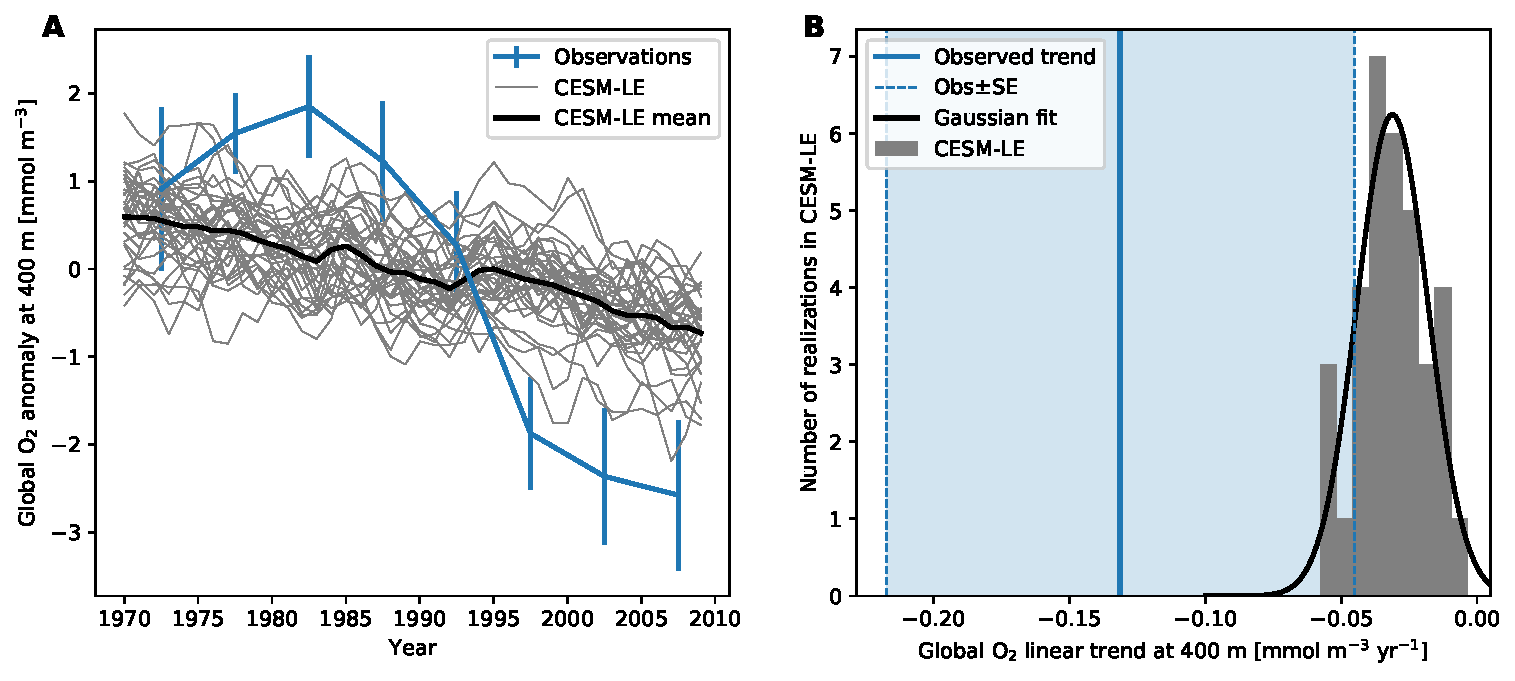
\includegraphics[width=1\textwidth]{obs-cesm-global-trends.pdf}
\caption{Global \ce{O2} trends from observations and CESM-LE.
(A) Globally average \ce{O2} concentration at the depth of 400m from 1970 to 2010.
The thin solid lines represent individual ensemble members of the CESM-LE, and the thick solid line is the ensemble mean.
Blue line is the pentad time series of objectively mapped \ce{O2} dataset based on the World Ocean Database \citep{Ito-Minobe-etal-2017}.
Error bars indicates one standard deviation of the pentad data.
(B) Histogram of linear \ce{O2} trend at 400~m.
The black line is a gaussian fit, and the blue solid is the observed trend; the dashed lines and shaded region show its uncertainty as measured by one standard error. }
\label{fig:test_trend_global}
\end{figure}
%-------------------------------------------------------------------------------

Figure \ref{fig:test_trend_global}a shows the comparison of the global \ce{O2} time series from the objectively-mapped historic \ce{O2} dataset \citep{Ito-Minobe-etal-2017} and CESM-LE.
They are both evaluated at 400~m depth for the period of 1970 to 2010.
The model and observations both show declining global \ce{O2} trends but the model appears to underestimate the global \ce{O2} trend evident in the observations.
The objectively mapped historic \ce{O2} dataset indicates a trend of $-0.13\pm0.09$~mmol~m$^{-3}$~yr$^{-1}$, where the uncertainty is the standard error of the regression coefficient.
The significant uncertainty arises because the observed time series substantially departs from a linear trend \citep{Santer-Mears-etal-2011}, which is due to the superposition of large, decadal-scale change evident as an apparently sinusoidal variation on Figure~\ref{fig:test_trend_global}a.
Figure \ref{fig:test_trend_global}b contrasts the observed and simulated linear trends of \ce{O2}.
The overlap between observations and the model is quite marginal.
The model underestimates the magnitude of the global \ce{O2} decline, as no single ensemble member reproduces the observed trend.
The ensemble mean trend ($-0.03$~mmol~m$^{-3}$~yr$^{-1}$) is a factor of 4 smaller in magnitude than the observationally-based estimate, but---due to the large uncertainty in the observations---the lower quartile trend ($-$0.04~mmol~m$^{-3}$~yr$^{-1}$) still overlaps with the upper bound of the observational uncertainty range (blue dashed line in Fig \ref{fig:test_trend_global}b).
The effect of natural variability, as represented by the spread of histogram in Figure~\ref{fig:test_trend_global}b, provides some sense of an expected range in the simulated trend, but there is a strikingly large difference between the spread in the ensemble members and the standard error of observed trend.
This indicates that the model may be severely underestimating the natural variability, and/or the existing observations lacks the spatial coverage to accurately determine the decadal fluctuation of global \ce{O2} time series.
Considering the poor data coverage in the historic observations, consistent and accurate monitoring of global \ce{O2} fields is a primary challenge.

%-------------------------------------------------------------------------------
\begin{figure}[tbp]
\centering
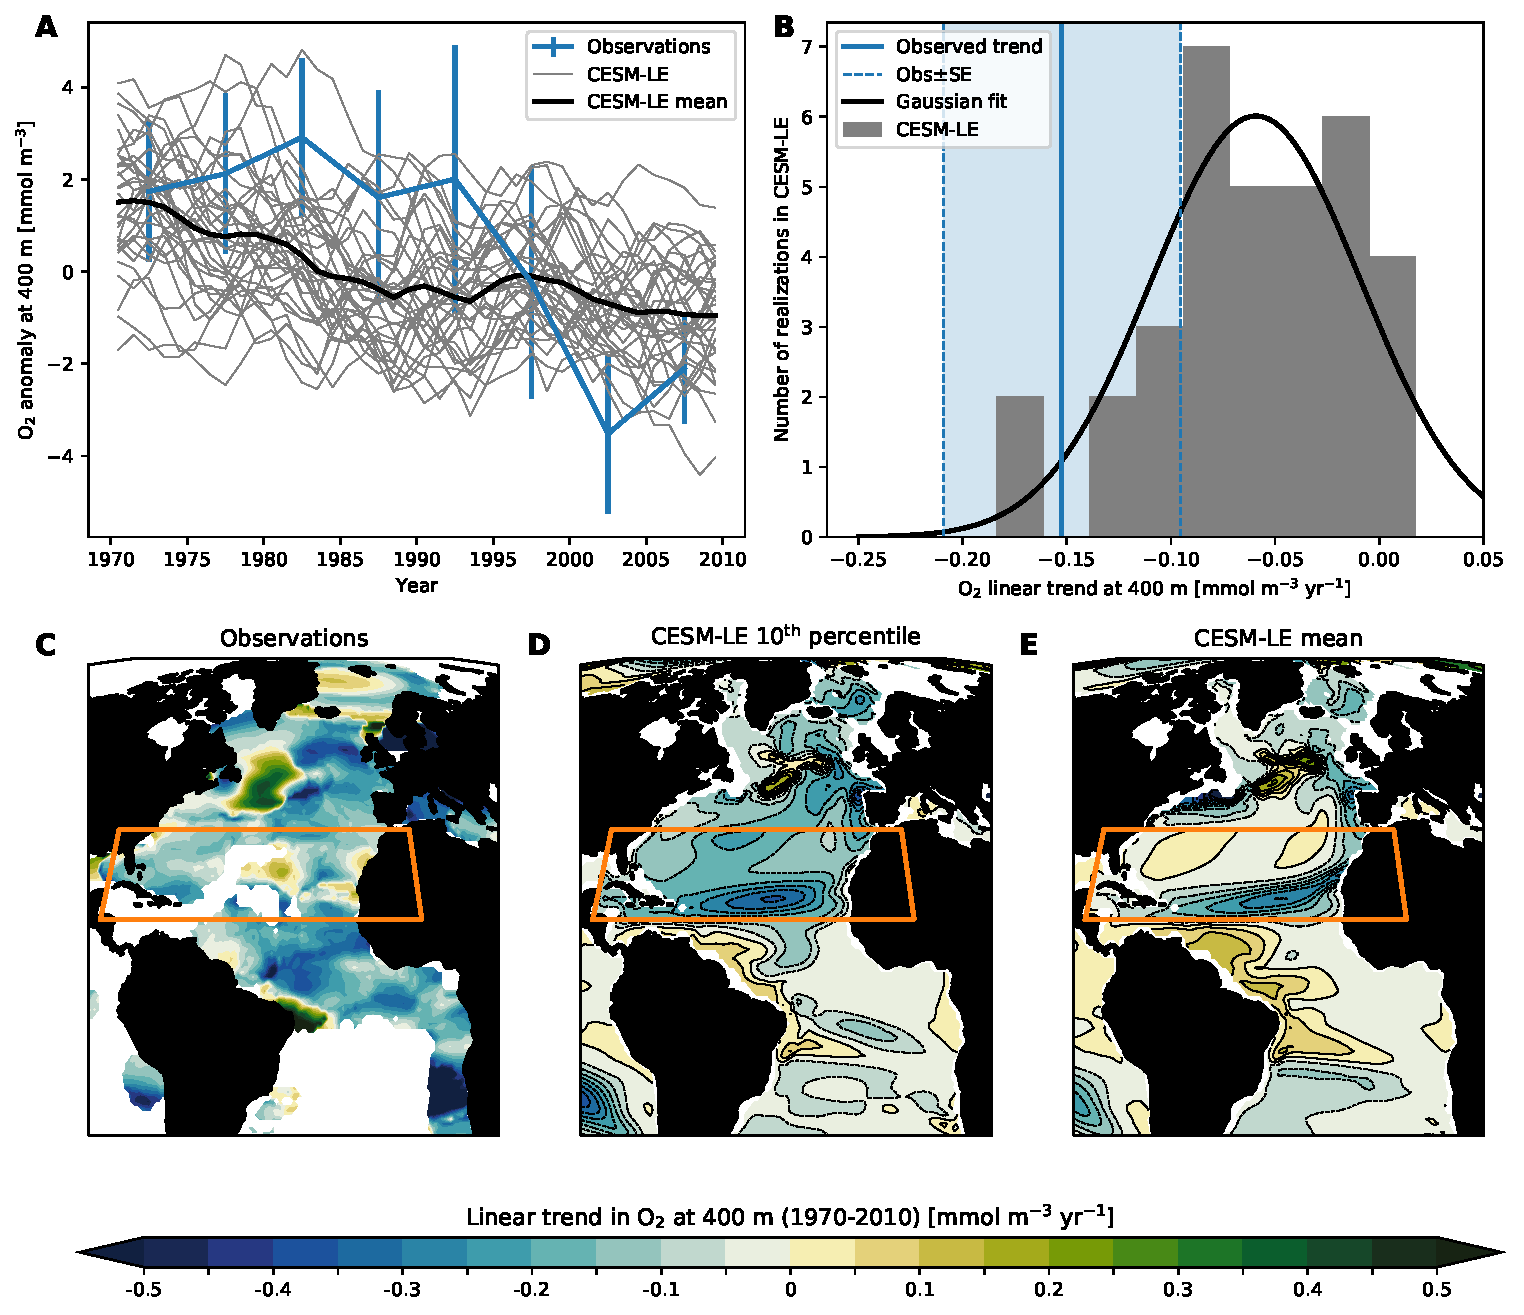
\includegraphics[width=1\textwidth]{obs-cesm-stna-trends.pdf}
\caption{\ce{O2} trends in the Subtropical North Atlantic (STNA; 15--35$^\circ$N) from observations and CESM-LE.
(A) STNA average \ce{O2} concentration at the depth of 400~m from 1970 to 2010.
The thin solid lines represent individual ensemble members of the CESM-LE, and the thick solid line is the ensemble mean.
The blue line is the pentad time series of objectively mapped \ce{O2} dataset based on the World Ocean Database \citep{Ito-Minobe-etal-2017}.
Error bar indicates one standard deviation of the pentad data.
(B) Histogram of linear \ce{O2} trend at 400~m.
The black line is a gaussian fit, and the blue solid is the observed trend; the dashed lines and shaded region show its uncertainty as measured by one standard error.
(C) Observed pattern of linear trend at 400~m depth from 1970 to 2010.
The trend is plotted for 1$^\circ$ $\times$ 1$^\circ$ grid cells within which at least 20-years of observations are available.
(D,E) 10th percentile and ensemble mean trend from the CESM-LE for the same depth and time period.
The orange box on the maps shows the region for which time series and trends are presented in panels (A) and (B).
}
\label{fig:test_trend_STNA}
\end{figure}
%-------------------------------------------------------------------------------

Assessing global trends places significant demands on observations for comprehensive coverage.
We might expect to be able to assess model behavior more robustly at regional scales.
Unfortunately, however, regions of intense interest, such as the thermocline of the Eastern Tropical Pacific, have been poorly sampled in the historical dataset, making the model-observation comparison difficult.
Even with the large observational uncertainty, \citet{Oschlies-Duteil-etal-2017} showed a persistent discrepancy in observed and simulated trends of \ce{O2} at the depth of 300~m, wherein the observations show trends that are consistently stronger than the models.
The subtropical North Atlantic, in contrast, has relatively high sampling density.
This is also a region where the models and observations agree relatively well (Figure \ref{fig:test_trend_STNA}).
Comparing the observed and simulated time series of \ce{O2} in the subtropical North Atlantic (15--35$^\circ$N), however, the ensemble mean again underestimates the long-term trend of \ce{O2}.
The observed linear trend (1970--2010) is $-0.15\pm0.06$~mmol~m$^{-3}$~yr$^{-1}$, where the uncertainty again is a standard error of the regression coefficient \citep{Santer-Mears-etal-2011}.
The ensemble mean trend ($-0.06$~mmol~m$^{-3}$~yr$^{-1}$) is a factor of 2.5 smaller than the observed trend.
However, a few ensemble members exceed the magnitude of observed deoxygenation in this region (as measured by the linear trend; Figure \ref{fig:test_trend_STNA}b).
Figures \ref{fig:test_trend_STNA}c--e compare the pattern of deoxygenation in the North Atlantic between observations, the 10th percentile composite from the CESM-LE, and the ensemble mean.
The ensemble mean clearly lacks the strong deoxygenation of the central subtropical gyre; however, there are a subset of ensemble members that exhibited trends nearly as intense as observed.
Further investigation is required to partition the roles of natural variability versus external forcing in driving observed \ce{O2} trends in this region; however, while this analysis emphasizes that natural variability can indeed play a substantial role in modulating trends, it also suggests that the CESM-LE and other CMIP5 models may underestimate deoxygenation.

%-------------------------------------------------------------------------------
\subsection{Nitrous oxide production}\label{loc:n2o}
%-------------------------------------------------------------------------------

Nitrous oxide (\ce{N2O}) affects climate in two distinct ways.
First, it is a strong greenhouse gas; thus, increasing \ce{N2O} concentrations in the troposphere have a strong effect on radiative forcing \citep{IPCC-2007}.
Second, since \ce{N2O} is relatively long-lived, it is mixed upward to the stratosphere, where it is a major contributor to the production of ozone depleting substances (\ce{NO} and \ce{NO2}) \citep{WMO-2011,Wuebbles-2009}.
Global-mean atmospheric \ce{N2O} concentrations have increased markedly from preindustrial levels, around 270~ppb, to near 330~ppb in 2017, mainly as a result of human activities \citep[][NOAA ESRL Global Monitoring Division,
 Boulder, Colorado, USA]{Forster-Ramaswamy-etal-2007}.
\ce{N2O} is produced naturally in soils and the ocean; agricultural, land use change, and industrial activities account for anthropogenic sources \citep{Denman-Brasseur-etal-2007}.
The IPCC Fourth Assessment Report estimated that the ocean accounts for about 35\% of the natural sources of \ce{N2O} to the atmosphere \citep{Denman-Brasseur-etal-2007}.

\ce{N2O} is produced by two microbially-mediated processes in the ocean: (1) under well-oxygenated conditions, microbes produce \ce{N2O} as a byproduct of  nitrification
($\ce{NH4}^+\rightarrow\ce{NO2}^-+\ce{NO3}^-$); and (2) at suboxic concentrations, denitrification produces \ce{N2O} as an intermediate during the conversion of nitrate to \ce{N2}
($\ce{NO3}^-\rightarrow\ce{NO2}^-\rightarrow\ce{N2O}\rightarrow\ce{N2}$)
\citep{Bange-Freing-etal-2010}.
When oxygen concentrations are very near zero, there is net consumption of \ce{N2O} during denitrification and little \ce{N2O} accumulation \citep{Bange-Freing-etal-2010}.
The \ce{N2O} yield of nitrification is sensitive to oxygen levels, however, increasing significantly as oxygen declines \citep[e.g.,][]{Santoro-Buchwald-etal-2011,Loscher-Kock-etal-2012}; thus, suboxic regions and surrounding hypoxic waters account for a substantial fraction of marine \ce{N2O} production \citep{Codispoti-2010}.

The expansion of suboxic and hypoxic waters (i.e., Figure~\ref{fig:volumes}) is very likely to impact the production and decomposition of \ce{N2O}.
Enhanced denitrification will lead to greater rates of fixed nitrogen loss from the ocean, with unknown implications on primary productivity.
The role of increasing denitrification on \ce{N2O} production remains even less clear; however, it is likely that \ce{N2O} yields from nitrification will increase, on average, as oxygen levels decline.
Moreover, oxygen loss in relatively shallow waters might enhance \ce{N2O} production because respiration rates are higher near the sunlit surface where primary productivity generates sinking organic matter \citep{Codispoti-2010}.
Our understanding of the collection of processes driving \ce{N2O} production, however, is insufficient to make definitive predictions.
Indeed, ocean warming may drive shifts in bacterial community composition, potentially impacting \ce{N2O} production \citep{Freing-Wallace-etal-2012}.
Nitrification has been shown to decrease at low pH, thus suggesting the potential for ocean acidification to impact \ce{N2O} production \citep{Beman-Chow-etal-2010}.
Modeling studies have projected decreased global \ce{N2O} emissions from the ocean, driven by reductions in primary productivity, which limits nitrification, and the direct effects of stratification, which traps \ce{N2O}  at depth \citep{Martinez-Rey-Bopp-etal-2015}.
These projections are highly uncertain, however, in part because models lack fully mechanistic representations of the processes mediating microbial transformations in the nitrogen cycle and the resultant \ce{N2O} yields; indeed, our empirical understanding of these processes is still developing \citep{Codispoti-2010}.

%-------------------------------------------------------------------------------
\subsection{Coastal deoxygenation}\label{loc:coastal}
%-------------------------------------------------------------------------------

Coastal ocean hypoxia has emerged as a growing threat to marine ecosystems and fisheries with high economic and societal value \citep{Diaz-Rosenberg-2008,McClatchie-Goericke-etal-2010}.
Oxygen decline in many coastal waters is driven by nutrient pollution.
The widespread use of chemical fertilizers and discharge of waste waters increases the nutrient content of surface waters on land; as these waters are discharged into coastal systems, elevated nutrient loads stimulate productivity \citep{Rabalais-Diaz-etal-2010}.
Additionally, fossil fuel combustion and agricultural activities are associated with increases in atmospheric deposition of nutrients to the ocean.
In particular, reactive nitrogen loads have increased substantially over the last century, enabled by industrial-scale artificial nitrogen fixation via the Haber-Bosch process \citep[e.g.,][]{Gruber-Galloway-2008}.
Nutrient pollution drives ``eutrophication'', wherein primary productivity increases, leading to oxygen declines as excess organic matter decomposes in subsurface waters.

Coastal habitats can be particularly vulnerable to future deoxygenation because of the compounding effects of nutrient runoff from the land and the large-scale ocean deoxygenation from the open ocean.
A major concern is that ocean deoxygenation drives declines in the oxygen content of offshore waters, lowering the baseline concentrations from which coastal eutrophication causes further oxygen depletion.
The CCS, for instance, is one of the most productive and biodiverse marine systems in the world \citep{Block-Jonsen-etal-2011,Carr-2001}.
In the CCS, like other coastal ocean upwelling systems, changes in the oxygen content are controlled by complex interactions between circulation and biogeochemistry, and show prominent fluctuations on interannual and decadal timescales both in observations and models \citep[section~\ref{loc:toe};][]{Bograd-Castro-etal-2008,Deutsch-Brix-etal-2011}.
Over the continental shelf region, where the marine ecosystem is most sensitive to low oxygen conditions, natural oxygen variations are associated with fluctuations in the strength of the coastal upwelling \citep{Connolly-Hickey-etal-2010,Chan-Barth-etal-2008}.
The subsurface waters in the offshore CCS region are charged with nutrient-rich, low-\ce{O2} waters, which can trigger high production of new organic matter as water upwells onto the continental shelf.
Coastal upwelling is driven by winds, which vary in intensity and seasonality due to both natural variability and anthropogenic climate warming.
The seasonal timing of upwelling-favorable winds has strong impact on the CCS system; for instance, \citet{Barth-Menge-etal-2007} demonstrated that delayed upwelling strongly impacted net primary productivity and food web structure in the CCS.
Theory suggests that the seasonal timing and intensity of upwelling-favorable winds is likely to change significantly in a warmer climate \citep{Bakun-1990}.
Indeed, consistent with this, a collection of the CMIP5 models suggest that upwelling-favorable winds in the CCS system will occur over a prolonged seasonal duration and become more intense at high latitudes \citep{Wang-Gouhier-etal-2015}.
The likely impacts of these changes on coastal ecosystems and marine biodiversity are not well-understood and merits further study.
It is clear, however, that changes in the properties of offshore source waters has a significant impact on hypoxia in the CCS system \citep{Grantham-Chan-etal-2004,Bograd-Castro-etal-2008}.
Moreover, the frequency of hypoxic events may be modulated by the slow, decadal changes in these subsurface water properties feeding the CCS upwelling.
\citet{Pozo-Buil-Di-Lorenzo-2017}, for instance, demonstrated that low-frequency changes in the oxygen levels of the CCS upwelling are driven by large-scale ocean circulation dynamics.
Oxygen anomalies are generated in regions well offshore in the Subarctic North Pacific and are advected across the basin in the North Pacific Current; these anomalies contribute to variations in hypoxia within the CCS on decadal to multi-decadal timescales \citep{Pozo-Buil-Di-Lorenzo-2017}.
Notably, the time required for the oxygen anomalies to cross the Pacific basin is about 10 years, indicating that with sufficiently robust observing capabilities, oxygen variability in the waters offshore the CCS might be predictable many years in advance.

In light of these dynamics, a major concern for the CCS and other similar coastal systems is the systematic and widespread depletion of oxygen in offshore waters.
While there is limited research on the future of coastal hypoxia taking into account different scenarios of coastal eutrophication and emissions, it is reasonable to expect large-scale oxygen declines to propagate down to local scales \citep{Bianucci-Fennel-etal-2015}.
Oxygen depletion in coastal upwelling systems happens naturally; however, as the oxygen levels decline offshore, hypoxic and anoxic events may become much more frequent and severe.
This is a critical consideration, especially since these coastal systems are profoundly important in both ecological and economic terms.


%-------------------------------------------------------------------------------
\subsection{Habitat of the future}\label{loc:MI}
%-------------------------------------------------------------------------------

The impact of ocean deoxygenation on marine conservation goals depends on the number and ecological roles of the species for which the loss of dissolved \ce{O2} crosses a critical biological threshold.
Based on compilations of lethal \ce{O2} levels from laboratory studies and the distribution of \ce{O2} in the ocean (i.e., Figure~\ref{fig:o2pdfs}ab), it would appear that the impact of deoxygenation will be confined to those species residing in the relatively small volumes of the oceans already at or near \ce{O2} levels below a nominal hypoxic level of $\sim$60~mmol~m$^{-3}$.
This view, however, neglects at least two critical facts about the provisioning of energy to aerobic marine organisms.
First, the energetic demands of organism metabolism rise with temperature.   Thus, as the oceans warms, even a constant \ce{O2} may not suffice to meet organisms' energetic demands.
Second, lethal thresholds measured in laboratory studies are carried out under conditions designed to quantify oxygen demand at the minimum metabolic rate in a state of rest.
Ecological survival in a realistic environments will typically require substantially more energy (and hence \ce{O2} supply) than would be indicated by the physiological survival evaluated by laboratory studies.
Indeed, among terrestrial taxa, active metabolic rates are found to be 1.5--7 times resting rates \citep{Peterson-Nagy-etal-1990}, suggesting that \ce{O2} thresholds for ecological survival may be several times higher than lethal thresholds would imply.

%-------------------------------------------------------------------------------
\begin{figure}[p]
\centering
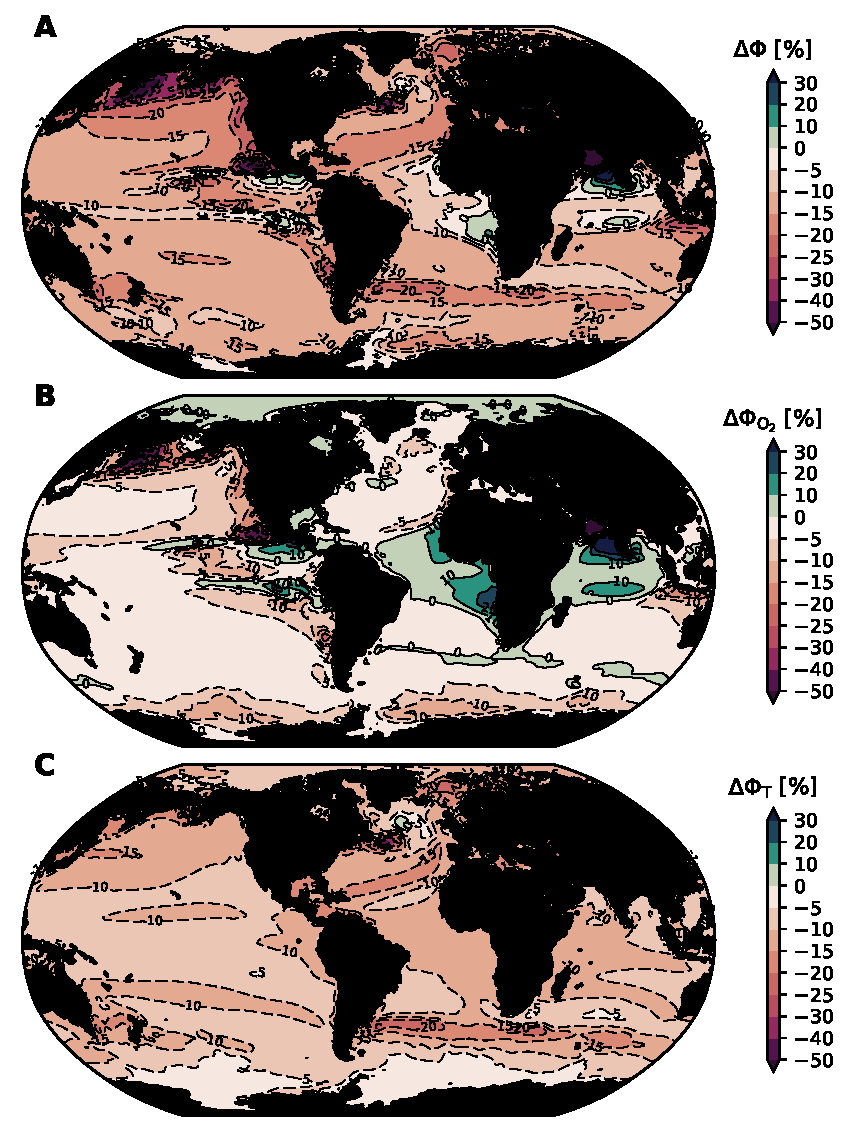
\includegraphics[width=0.75\textwidth]{metabolic-index-change-map.pdf}
% generated by: plot_global_timeseries.ipynb
\caption{Relative change in the Metabolic Index ($\Phi$; equation~\ref{eqn:MI}) at year 2100 over the top 400~m of the ocean according to the bias-corrected, CMIP5 ensemble mean:
(A) the total relative change in $\Phi$, i.e. ${\Delta\Phi = 100\times(\Phi^{2100}-\Phi^{2000})/\Phi^{2000}}$; (B) the relative change in $\Phi$ due purely to changes in \ce{O2}; (C) the relative change in $\Phi$ due purely to changes in temperature.
The relative change has no dependence on $A_o$ or $B^n$; the total and temperature-driven components of change depend on $E_o$.
For this presentation, we have used $E_o = 0.4$, which is the mean of the several taxa for which $E_o$ has been characterized \citep{Deutsch-Ferrel-etal-2015}.
}
\label{fig:MI-change-map}
\end{figure}
%-------------------------------------------------------------------------------

%-------------------------------------------------------------------------------
\begin{figure}[p]
\centering
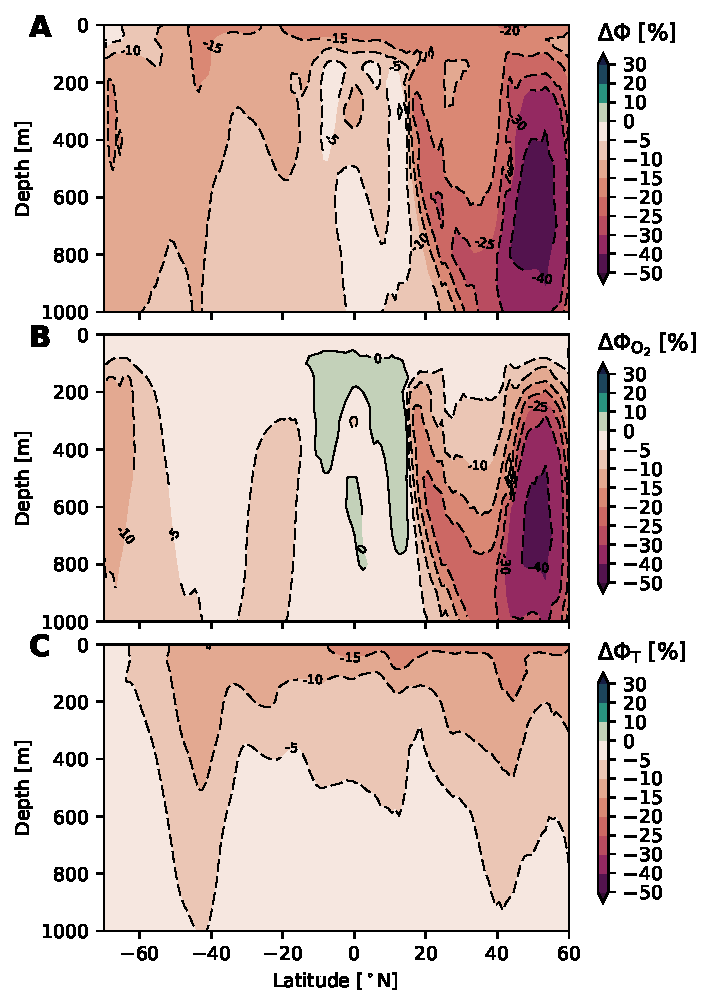
\includegraphics[width=0.6\textwidth]{metabolic-index-change-zonal.pdf}
\caption{Zonal mean relative change in the Metabolic Index ($\Phi$; equation~\ref{eqn:MI}) at year 2100 according to the bias-corrected, CMIP5 ensemble mean:
(A) the total relative change in $\Phi$; (B) the relative change in $\Phi$ due purely to changes in \ce{O2}; (C) the relative change in $\Phi$ due purely to changes in temperature.
See the caption of Figure~\ref{fig:MI-change-map} for further details.
}
\label{fig:MI-change-zonal}
\end{figure}
%-------------------------------------------------------------------------------

An ecophysiological framework has recently been developed to investigate metabolic habitat constraints in light of these factors, for the contemporary, past, and future oceans.
The framework is built on a Metabolic Index ($\Phi$), which can be calibrated with laboratory and biogeographic data \citep{Deutsch-Ferrel-etal-2015}.
The Metabolic Index uses physiological data on hypoxia tolerance across a range of temperatures and body sizes to calibrate the ratio of oxygen supply ($S$) to an organism's resting demand ($D$).
The supply of oxygen is a function of the ambient partial pressure of oxygen ($p\ce{O2}$) and the efficiency with which an organism can acquire and utilize \ce{O2}.
This can be written as $S = \alpha_S B^{\delta}p\ce{O2}$, where $\alpha_S$ is a mass-normalized coefficient expressing the rate of gas transfer between an organism and its environment and $B^{\delta}$ is the scaling of supply with biomass $B$ \citep{Piiper-Dejours-etal-1971}.
Resting metabolic demand can be expressed as $D = \alpha_D B^{\epsilon}\mathrm{exp}(-E_o/k_B T)$, where $\alpha_D$ is a taxon-specific basal metabolic rate, $B^\epsilon$ is the scaling of this rate with biomass, $E_o$ is the temperature dependence, and $k_B$ is the Boltzmann constant \citep{Gillooly-Brown-etal-2001}.
We construct the Metabolic Index as the ratio $S/D$:
\begin{equation}
\Phi = A_o B^n  \frac{p\ce{O2}}{\mathrm{exp}(-E_o/k_B T)}
\label{eqn:MI}
\end{equation}
where $A_o=\alpha_S\alpha_D$ is the ratio of rate coefficients for gas exchange (\ce{O2} supply) and minimum metabolic rate (\ce{O2} demand) and $n$ is the difference between the scaling exponents applied to body size ($B$) for \ce{O2} supply and demand.
If $\Phi$ falls below a critical threshold value of 1, organisms must either suppress aerobic activity or initiate anaerobic metabolism, conditions that are physiologically unsustainable.
Conversely, values above 1 enable organismal metabolic rates to increase by a factor of $\Phi$ above resting levels, permitting critical activities such as feeding, defense, growth, and reproduction.
Thus for a given environment, $\Phi$ estimates the ratio of maximum sustainable metabolic rate to the minimum rate necessary for maintenance for a given species.

For marine animals, this ratio of active to resting energetic demand can be inferred by mapping $\Phi$ alongside the species biogeographic distribution \citep{Deutsch-Ferrel-etal-2015}.
Among all taxa studied to date ($n\approx20$), species geographic range boundaries are found to coincide with Metabolic Index values of between 1.5--7, identical to the range predicted by terrestrial energetic demands.
Where the ocean's supply of \ce{O2} falls below this critical threshold, termed $\Phi_{crit}$, the Metabolic Index acts as a fundamental energetic barrier for species habitat.
In other words, if climate warming and \ce{O2} loss reduce the Metabolic Index for an organism below its species-specific $\Phi_{crit}$, the environment would no longer have the aerobic capacity to support the organism's energetic requirements.
The Metabolic Index can therefore be used to quantify the loss of aerobically viable habitat for marine animals due to the combined effects of climate warming and attendant \ce{O2} loss.
It can also be used to track the relative role of each stressor in governing viable habitat across space and depth.
This is particularly useful as the magnitudes of warming and deoxygenation can differ dramatically among regions of the ocean (Figures~\ref{fig:cesm-temp-change} and \ref{fig:cesm-thermocline-o2-change}).

Figure~\ref{fig:MI-change-map} shows the relative change in $\Phi$ over the top 400~m of the ocean for an organism with an average metabolic temperature sensitivity ($E_o = 0.4$).
There are widespread declines in $\Phi$ over most of the ocean; only in small pockets in the tropics does $\Phi$ modestly increase.
Relative changes in $\Phi$ in excess of 40\% are found in the Subarctic North Pacific, suggesting that this region may be particularly impacted by climate change and deoxygenation.
Figures~\ref{fig:MI-change-map}b and \ref{fig:MI-change-map}c demonstrate why it is important to consider changes in temperature and oxygen together.
Figure~\ref{fig:MI-change-map}b shows the change in $\Phi$ that would be realized if oxygen was changed in isolation.
The subarctic North Pacific stands out again in this field, but much of the tropics where models simulate oxygen increases show improvements in $\Phi$.
Temperature-driven reductions in $\Phi$, however, are nearly ubiquitous, which we might expect from the distribution of surface warming (Figure~\ref{fig:cesm-temp-change}).
The fact that metabolic rates scale with temperature means that even present-day distributions of oxygen may not be sufficient to meet metabolic demands in some regions in the future.
The depth structure of changes in $\Phi$ are shown in Figure~\ref{fig:MI-change-zonal}.
Strong reductions in $\Phi$ are predicted for the upper 1000~m of ocean over much of the high-latitude northern hemisphere (Figure~\ref{fig:MI-change-zonal}a).
The oxygen-driven and temperature-driven changes in the zonal-mean $\Phi$ have a fundamentally different structure (Figure~\ref{fig:MI-change-zonal}bc).
Oxygen-driven changes are most intense below 200~m, which is where oxygen depletion is most pronounced (Figure~\ref{fig:zonal-mean-section}).
The modest increases in oxygen in the tropical thermocline yield oxygen-driven increases in $\Phi$ locally.

The restrictions of habitat imposed by the need to balance \ce{O2} supply and demand vary across species, and the tightening of those constraints during ocean warming will depend critically on the relative magnitude and patterns of ocean warming and deoxygenation.
Thus, a generalized prediction of the responses of marine species to ongoing global change must rely on an adequate characterizations of species diversity with respect to Metabolic Index traits, and on a regional basis, since temperatures and \ce{O2} levels can operate in both synergistic and counteracting directions.


%-------------------------------------------------------------------------------
\begin{sidewaysfigure}[p!]
\centering
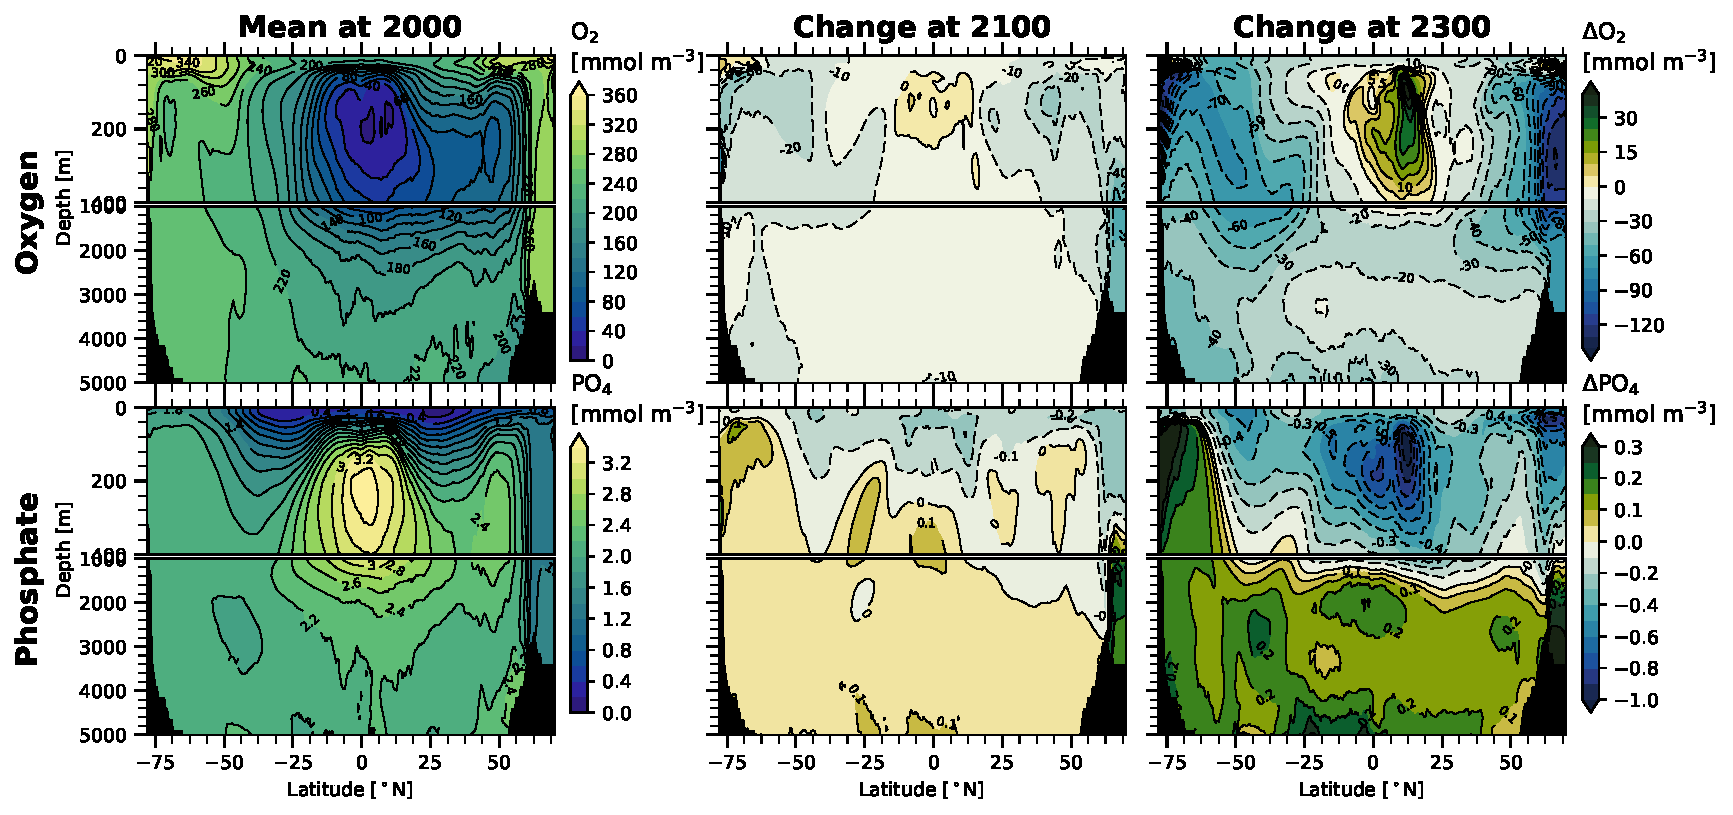
\includegraphics[width=0.8\textwidth]{global-zonal-mean-2300.pdf}
\caption{Zonal mean oxygen (top) and phosphate (bottom) in a CESM1-BGC simulation, averaged over 1995--2005 (left column).
The middle column shows the change in zonal mean oxygen and phosphate at 2100 (2090--2100 minus 1995--2005); the right column shows the change at 2300 (2280--2300 minus 1995--2005).}
\label{fig:2300}
\end{sidewaysfigure}
%-------------------------------------------------------------------------------

%-------------------------------------------------------------------------------
\section{Action}
%-------------------------------------------------------------------------------

Ocean oxygen concentrations are strongly linked to ocean heat content (Figure~\ref{fig:o2-heat}); therefore, substantial deoxygenation is unavoidable without mitigating climate change.
Even in the best circumstances, some degree of continued ocean warming is unavoidable and, given the longevity of perturbations to atmospheric \ce{CO2} \citep{Archer-Kheshgi-etal-1997}, current emissions commit the climate system to sustained alteration.
Efforts to conserve marine ecosystems must account for the synergistic effects of multiple variables changing simultaneously \citep[e.g.,][]{Brewer-Peltzer-2009,Portner-2010,Deutsch-Ferrel-etal-2015,Boyd-Lennartz-etal-2014}.
Indeed, ocean warming, acidification, oxygen loss, and reductions in primary productivity are key components of a suite of multiple stressors effecting ecosystem change.
Specifically in the context of ocean deoxygenation, we can frame our discussion about mitigation actions around two questions.
(1) What are the consequences if nothing is done to mitigate climate warming?
(2) What are the benefits of mitigation actions?

Perspective on the risks of inaction is provided by considering what happens after 2100.
Warming over the 21st century is very likely to lead to disruptive consequences; an examination of model projections under extended RCP8.5 scenarios out to 2300, however, suggest that long-term effects of unmitigated human-driven climate change could be catastrophic.
Figure~\ref{fig:2300} presents a zonal-mean view of oxygen and phosphate in the present-day climate as well as changes to these fields at 2100 and 2300.
The scenario used to integrate the model out to 2300 follows historical and then the RCP8.5 forcing out to 2100; this entails an increase of atmospheric \ce{CO2} from 285~ppm at 1850 to about 940~ppm at 2100---\ce{CO2} then continues to increase to 1962~ppm at 2300.
The impacts on ocean oxygen involve a strong amplification of the pattern of change at 2100: high latitude regions show substantial oxygen declines.  While there are increases in oxygen within the tropical thermocline, those regions remain below the biological thresholds of habitability for many species.
The magnitude of these changes is shocking: the zonal-mean changes in oxygen concentrations at high latitudes approach and even exceed 100~mmol~m$^{-3}$; the entire deep ocean substantially deoxygenates (Figure~\ref{fig:2300}, top right).

The changes in oxygen at 2300 are associated with a massive redistribution of nutrients.
The surface ocean becomes strongly depleted in phosphate, whereas the deep ocean phosphate inventory increases; this increase is consistent with growth of the remineralized nutrient inventory and thus $AOU$.
Stratification reduces the vertical fluxes of phosphate from depth into the surface ocean over much of globe; however, reductions in sea ice and changes in upwelling in the Antarctic Zone of the Southern Ocean promote high productivity there, which effects a more complete transfer of nutrients from the upper ocean to deep waters \citep{Primeau-Holzer-etal-2013}.
The surface depletion of nutrients will drive declines in primary productivity, dramatically reducing the flow of energy into marine ecosystems.
This is likely to strongly reduce potential fisheries yields \citep{Stock-John-etal-2017,Pauly-Christensen-1995} and may lead to a fundamental reorganization of ocean food webs \citep{Hoegh-Guldberg-Bruno-2010}.

The depletion of oxygen at 2300 represents a severe contraction of viable habitat on the basis of the metabolic constraints discussed in section~\ref{loc:MI}.
Indeed, these changes are similar in structure to simulations conducted with CESM of ocean climate change at the end-Permian extinction event ($\sim$252 million years ago); analysis of these simulations indicates that warming and deoxygenation can account for extinction patterns (unpublished), leading to a haunting conclusion: human-induced warming is driving patterns of change that are consistent with those of the most severe crisis in the history of life on Earth.

A comparison between 2100 and 2300 confirms that the severity of deoxygenation and its consequences will grow in the absence of efforts to mitigate climate change.
However, it is also important to consider that climate change is essentially irreversible on human timescales.
\citet{Solomon-Plattner-etal-2009} demonstrated this using an Earth System Models of Intermediate Complexity; they conducted idealized forcing scenarios, wherein emissions were instantaneously ceased following a period of increase similar to that in RCP8.5.
Carbon dioxide concentrations begin to decline following the cessation of emissions, but the carbon perturbation requires several centuries to fully dissipate \citep{Archer-Kheshgi-etal-1997,Archer-Brovkin-2008}.
Moreover, even as radiative forcing due to \ce{CO2} begins to decline, the ocean continues to warm, but at a slower rate; thus surface temperatures remain elevated for more than 1,000 years following an abrupt stop in emissions \citep{Solomon-Plattner-etal-2009}.
Few studies have explicitly examined irreversibility in the context of ocean biogeochemistry and ecology; this is an important area for further research.

The long persistence timescales of ocean deoxygenation drivers suggests that early action to mitigate climate change will maximize benefit.
The benefits of mitigation can be quantified in terms of the reduced magnitude of change in some state variable (i.e., preserving oxygen content) or in  delaying impacts, providing time for adaptation.
\citet{Henson-Beaulieu-etal-2017}, for instance, examined the ToE of anthropogenic signals in sea surface temperature, pH, primary productivity, and interior oxygen distributions; by comparing RCP8.5 to a ``mitigation scenario'' (RCP4.5); they demonstrate benefits of mitigation in terms of reduced areal extent and delayed emergence of stressors.
The benefits of delayed impacts can include time for organisms to adapt or migrate to avoid impacts \citep{Henson-Beaulieu-etal-2017}.
Understanding how delayed emergence will effect the structure and function of marine ecosystems is very complicated, however; thus, it is not clear whether the difference between RCP8.5 and RCP4.5 is a meaningful one from an ecological perspective.
Moreover, in cases where species are already living near the edge of their ecophysiologically-viable envelop, such as at high latitudes, there may be no refuge from which to avoid climate change impacts.
These considerations are critical to developing better quantifications of the avoided impacts of climate change associated with mitigation efforts.
A few studies have framed analyses of ESMs in this context \citep[e.g.,][]{Krumhardt-Lovenduski-etal-2016}, but this is an area where much more additional research is needed.

Finally, while climate change mitigation is critical to avoiding deoxygenation, investments in observing systems and modeling capabilities may help provide adaptive capacity.
There is good reason to believe, for instance, that oxygen distributions can be forecast years in ahead in some regions \citep[e.g.,][]{Pozo-Buil-Di-Lorenzo-2017}, possibly enabling advanced warming of especially low-oxygen periods.
Humanity is changing marine ecosystems faster than we can understand them; there is strong role for science in enabling informed decisions about managing this global-scale impact.

%-------------------------------------------------------------------------------
\section{Conclusions}
%-------------------------------------------------------------------------------

Ocean deoxygenation presents a compelling case-study demonstrating the intricate interrelationships characterizing Earth system function.
The planetary energy balance is determined by the composition of the atmosphere, including, most importantly, carbon dioxide.
Carbon is the primary currency of life on Earth; the flow of energy and material through the biosphere plays a role in regulating atmospheric composition and the radiative balance controlling climate.
Humans, however, have released massive quantities of geologically-sequestered \ce{CO2}, disrupting this balance, trapping more heat and warming the planet.
The ocean is the dominant heat reservoir in the climate system and thus absorbs most of this anomalous heat.
Ocean warming drives deoxygenation by directly impacting the gas solubility: warmer waters hold less oxygen.
Furthermore, warming causes the ocean to become more stratified, inhibiting vertical exchange between surface and deep waters---and thereby reducing the supply of oxygen to the ocean interior.

Ocean ecosystem are built on the energy harvested from the sun during photosynthesis---the same process that contributes to regulation of the carbon cycle and produces most of the oxygen in the Earth system.
The flow of energy contained in photosynthetically-produced organic matter and the oxygen necessary to respire it have enabled the wide diversity of animal life on the planet.
The carbon cycle is coupled to the cycles of nutrients such as nitrogen and phosphorus, required building blocks of organic matter.
Oxygen mediates the return of these nutrients from their organic forms to those that refuel photosynthesis.
In this manner, the global biosphere consists of an interconnected, metabolic network in which many of the key linkages are mediated by microbial transformations.
Oxygen exerts strong control across two critical components of this network.
It is a fundamental requirement for animal life and it regulates microbial metabolism, affecting which transformations take place.

Earth system models predict substantial deoxygenation over the 21st century, with a rapid acceleration in oxygen loss expected in the coming decades.
These models suggest that deoxygenation will be strongest at high latitudes, where the effects of solubility and stratification are reinforcing.
The loss of oxygen in the tropics, according to these models, is tempered by opposing drivers: reductions in solubility are projected to be offset somewhat by reductions in respiration, the latter caused primarily by changes in circulation.
Most ESMs project increases in oxygen in the tropical thermocline over the 21st century.
These increases occur in regions where oxygen is already very low in the present climate---and the models also tend to predict increases in hypoxic and suboxic water volumes, suggesting that while oxygen concentrations may increase in the core of oxygen minimum zones, these zones will still expand.
However, ESMs struggle to accurately simulate present-day oxygen distributions in the tropics; thus, the future of oxygen in these regions of the ocean is somewhat uncertain.
Moreover, an observationally-based relationship between oxygen loss and ocean heat content anomaly suggests that the model projections may be too conservative: the observed relationship would suggest greater rates of oxygen loss than simulated by the models.

The changes projected in dissolved oxygen over the next century are likely to force dramatic changes in marine ecosystems.
Simulations of the ``deep future'' (out to 2300) project changes to oxygen and nutrient distributions that would yield catastrophic consequences for marine life.
More research is needed to fully quantify how climate change mitigation can benefit conservation.
However, there is virtually no uncertainty that the present climate trajectory will lead to substantial oxygen loss from the oceans, resulting in profound impacts to ocean ecosystems and biogeochemistry.
Animals reliant on aerobic metabolisms will experience habitat contraction as regions with oxygen below hypoxic limits expand.
Ocean microbial communities will be affected, leading to altered nutrients cycles: rates of fixed nitrogen loss from the ocean will increase; \ce{N2O} production and release is likely to change, though by how much is substantially uncertain.

The scale of the deoxygenation problem is truly planetary: the ocean occupies $\sim$70\% of the Earth's surface; as anthropogenic warming proceeds, oxygen concentrations will decline---leaving a nearly ubiquitous imprint of human-activity on this vast ecosystem.
The potentially profound changes in ocean habits and biogeochemical cycles associated with deoxygenation provide dramatic illustration of the degree to which humanity is a dominant influence on Earth's ecosystems \citep{Vitousek-Mooney-etal-1997}.

%-------------------------------------------------------------------------------
\bibliography{references.bib}
%-------------------------------------------------------------------------------

\end{document}
